\chapter{Aplicación Virtual Force Field}
\label{cap:capitulo6}
Como ya se ha explicado, otra de las aplicaciones que se va a desarrollar consiste en navegación usando el algoritmo VFF mediante el uso de máquinas de estados.

Para desarrollar esta aplicación, el proceso se dividirá en dos partes: desarrollo del algoritmo VFF e implementación de dicho comportamiento
en una máquina de estados que genere ubicaciones aleatorias.

\section{Campo de fuerzas virtuales (VFF)}
\label{sec:VFF}

El algoritmo de movimiento mediante campo de fuerzas virtuales o \textit{virtual field force} consiste en permitir el movimiento a través de un lugar avanzando gracias a
objetivos temporales (como si fueran balizas) y esquivando los obstáculos entre la posición del robot y el objetivo mediante la fuerza repulsiva generada por las medidas
de los distintos sensores al percibir dichos obstáculos.\\

Este algoritmo se basa en dos partes principales: la fuerza repulsiva (inversamente proporcional a la distancia con los obstáculos) y la
fuerza atractiva (dirección al objetivo). Para obtener ambas fuerzas serán necesarios dos sensores: láser (fuerza repulsiva) y odometría (fuerza atractiva).\\

\subsection{Diseño del circuito y escenario}
\label{subsec:dis_bloques_VFF}

El circuito para este comportamiento consistirá de dos ramas principales, una para cada fuerza, y la unión de estas ramas mandando una velocidad final tanto lineal como angular.\\

En la rama superior esta el sensor láser junto con un bloque para obtener una única medida como resultado de todas las medidas del láser. En la inferior se encuentra el sensor
\textit{odom}, que da la posición del robot en las coordenadas del mundo simulado.
Esta medida se pasa a dos bloques: el generador de objetivos (bloque que envía el objetivo actual
y, en caso de haber llegado, envía el siguiente dentro de una lista) y el bloque que se encarga de calcular la fuerza atractiva.

Ambas ramas se juntan en un bloque que las suma teniendo en cuenta sus valores de influencia (la repulsiva debe influir más que la atractiva para evitar colisiones por
roce) y se envían como velocidades al bloque MotorDriverROS2 (\ref{sec:motordriverros2}).
\begin{figure} [H]
    \begin{center}
        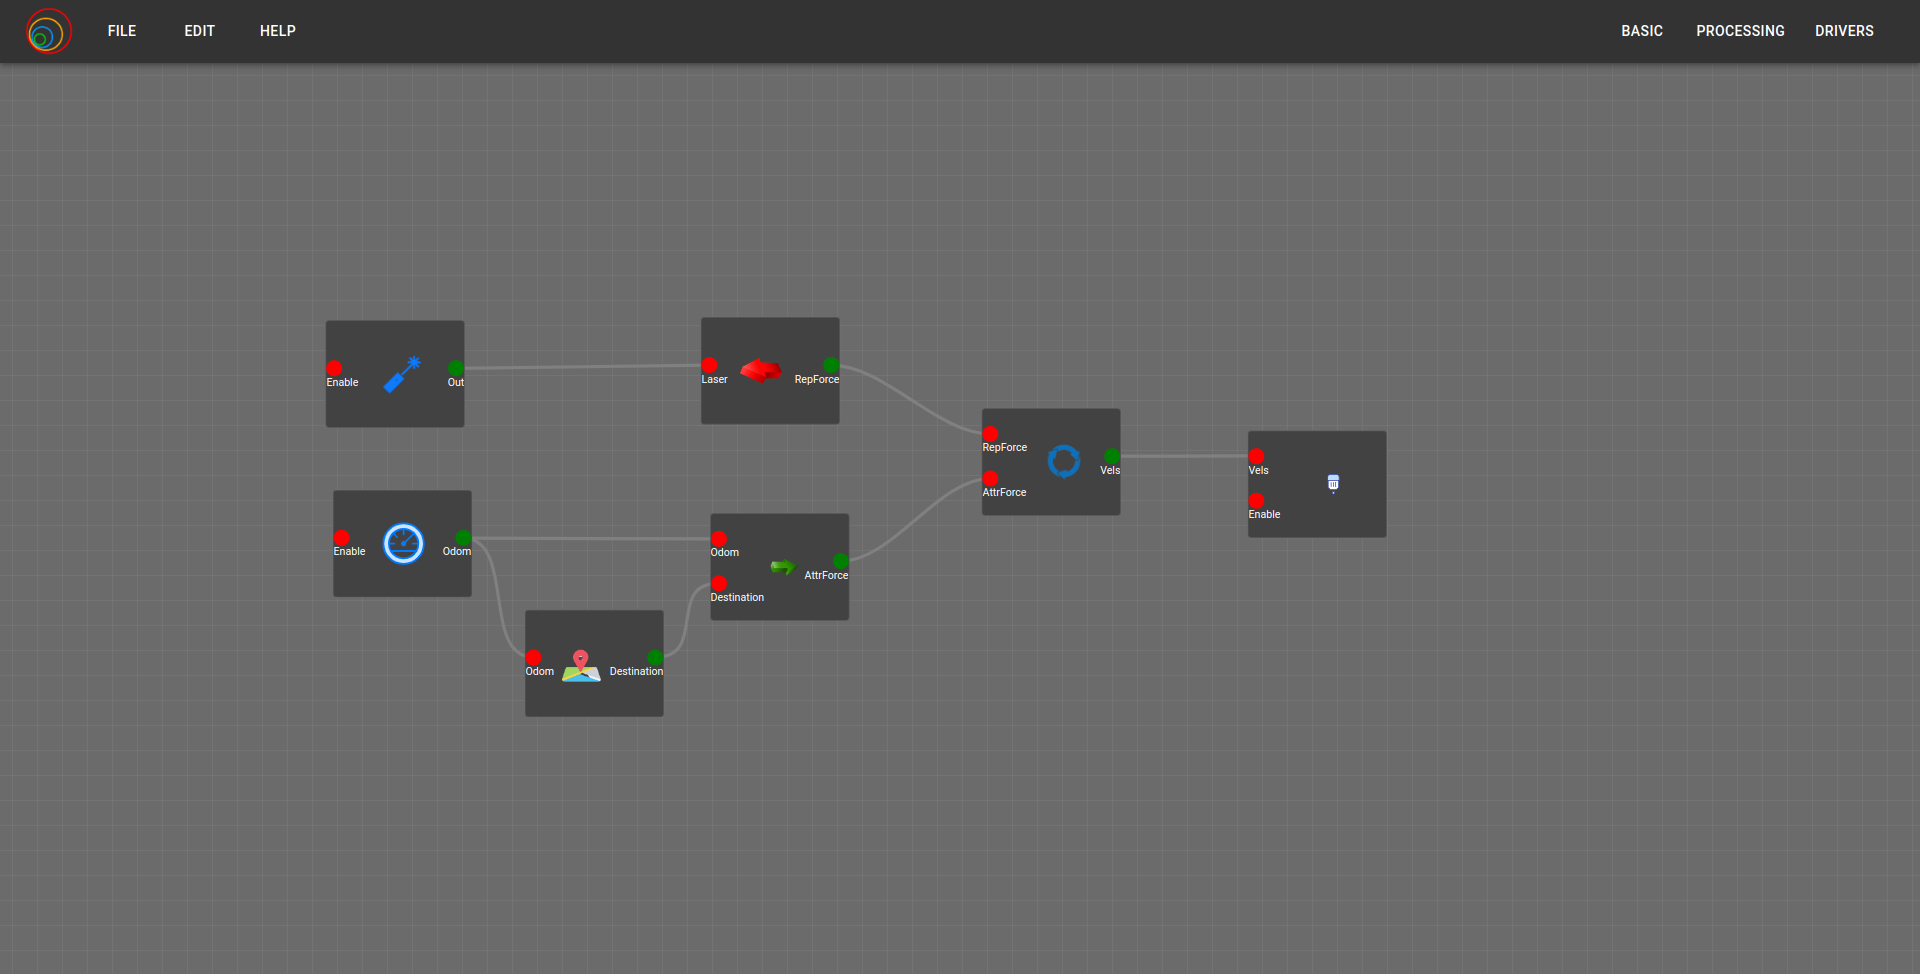
\includegraphics[width=12cm]{figs/c6/VFF_circ.png}
    \end{center}
    \caption[Circuito VFF]{Circuito del algoritmo VFF.}
    \label{fig:VFF_circ}
\end{figure}
El escenario de pruebas consistirá en un circuito creado a base de bloques cúbicos como muros con algunas barras rojas (cubos rectangulares) horizontales que marcan
aproximadamente dónde se encuentran los objetivos. Hay una zona en la que no hay practicamente borde para comprobar que la fuerza atractiva fuese lo suficiente fuerte
como para no desviarse al encontrar un hueco en uno de los lados.

\begin{figure} [H]
    \begin{center}
        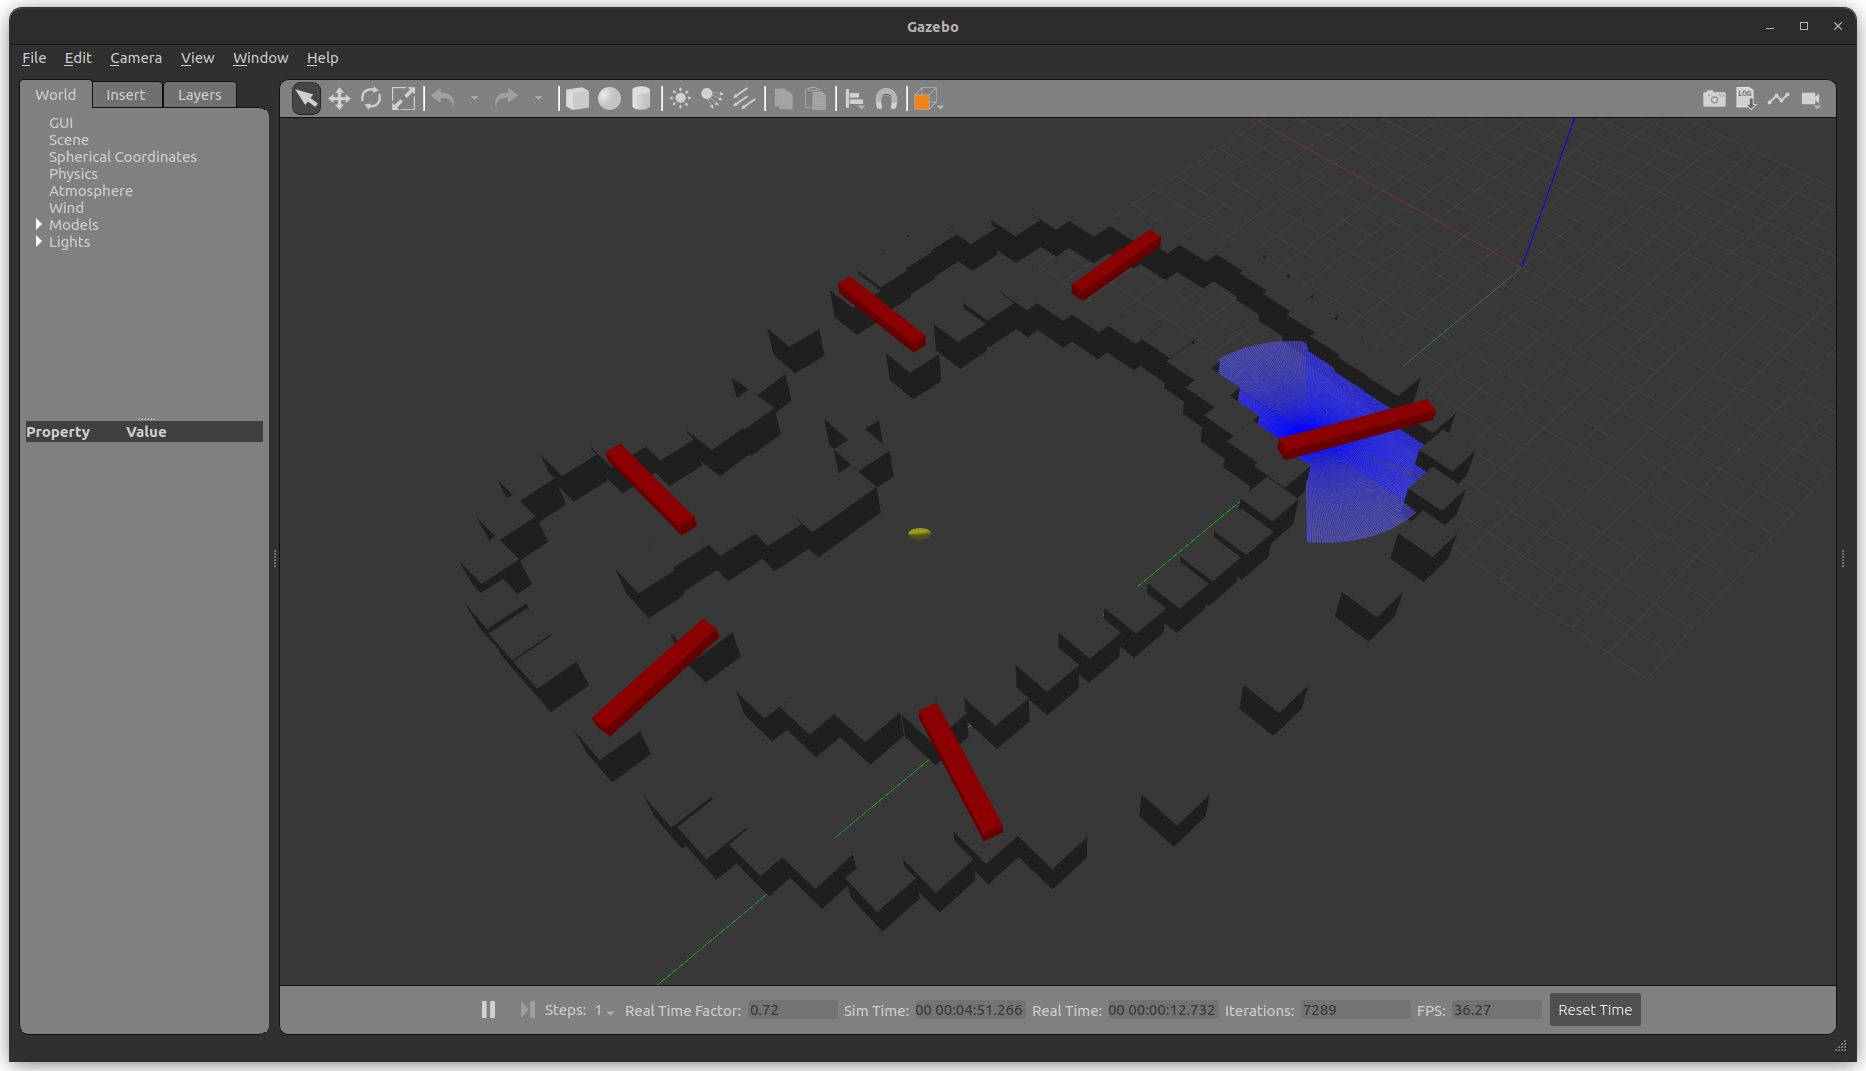
\includegraphics[width=12cm]{figs/c6/VFF_world.png}
    \end{center}
    \caption[Mundo para VFF]{Mundo gazebo para probar el algoritmo VFF.}
    \label{fig:VFF_world}
\end{figure}

\subsection{Bloques específicos}
\label{subsec:spec_bloques_VFF}

El primer bloque nuevo específico de esta aplicación es el que transforma las medidas del láser a un valor único.
Para que la información del láser sea más facilmente manipulable, se ha crea una función \textit{parse\_laser\_data()} que almacena cada medida del láser
en un array de tuplas junto al ángulo que dicha medida representa.\\

Después se recorre el array de tuplas para obtener vectores que representen el valor del eje X e Y para cada medida del láser. Ésto se hace multiplicando la medida
original (hipotenusa) por el seno o coseno del ángulo. Después se guarda en un nuevo array de tuplas para cada par de valore (x,y).\\

Ahora para calcular la fuerza final se recorre el array de medidas vectoriales sumando los valores inversos, es decir, el valor absoluto de la división de un valor
entre la medida, permitiendo que cuanto más cercano (menor sea la medida) mayor influencia tenga en el resultado de fuerza repulsiva final. En el caso del eje X, sólo
hay que comprobar que la medida sea distinta de 0, mientras que en el caso del eje Y hay que evitar medidas superiores a 10, ya que es el límite del sensor y
sumaría \textit{inf} (infinito).

\begin{code}[H]
    \begin{lstlisting}[language=python]
    def parse_laser_data (laser_data):
        laser = []
        for i in range(len(laser_data)):
            dist = laser_data[i]
            angle = math.radians (i)
            laser += [(dist, angle)]
        return laser
    
    def getObs_xy(laser):
        laser2 = parse_laser_data(laser)
        laser_vectorized = []
        for d, a in laser2:
            if(a == 0):
                x = 10
                y = 10
            else:
                x = d * math.cos (a) * -1
                y = d * math.sin (a) * -1
            v = (x, y)
            laser_vectorized += [v]
    \end{lstlisting}
\end{code}
\begin{code}[H]
    \begin{lstlisting}[language=python]
        obsx = 0
        obsy = 0    
        amortiguacion = 1   #Mayor amortiguacion, mas valen los valores lejanos
        pico = 1            #Mayor pico, mas valen los valores cercanos a cero
        for i in range(int(len(laser_vectorized)/2)):
            if(laser_vectorized[i][0] != 0):
                obsx -= pico*abs(math.atan(amortiguacion/(laser_vectorized[i][0])))
            if(i<90):
                if(laser_vectorized[i][1] != 0 and laser_vectorized[i][1] < 10):
                    obsy -= pico*abs(math.atan(amortiguacion/(laser_vectorized[i][1])))
            else:
                if(laser_vectorized[180+i][1] != 0 and laser_vectorized[180+i][1] < 10):
                    obsy += pico*abs(math.atan(amortiguacion/(laser_vectorized[180+i][1])))
        return obsx, obsy

    def main(inputs, outputs, parameters, synchronise):
        reduction = 1/50
        try:
            while 1:    
                measures = inputs.read_array("Laser")
                if measures is not None:
                    obsX, obsY = getObs_xy(measures)
                    outputs.share_array("RepForce", [obsX/50, obsY/50])
    \end{lstlisting}
    \caption[Funciones para obtener la fuerza repulsiva]{Funciones para obtener la fuerza repulsiva.}
    \label{cod:parse_laser_data}
\end{code}

En cuanto a la fuerza atractiva, se debe usar la posición actual del robot y la posición que se ha marcado como destino. 

Para ello se usará la plantilla para bloques sensores que se planteó en el capítulo 4 (\ref{cod:bloques_drivers_sensors_node_class} y \ref{cod:bloques_drivers_sensors_main_general}),
modificando el tipo de mensaje, ya que el \textit{topic /odom} tiene el tipo de mensaje \textit{nav\_msgs/msg/Odometry}, cuyos parámetros podemos comprobar mediante el comando 
``\lstinline|ros2 interface show nav_msgs/msg/Odometry|" con el siguiente resultado:
\begin{figure} [H]
    \begin{center}
        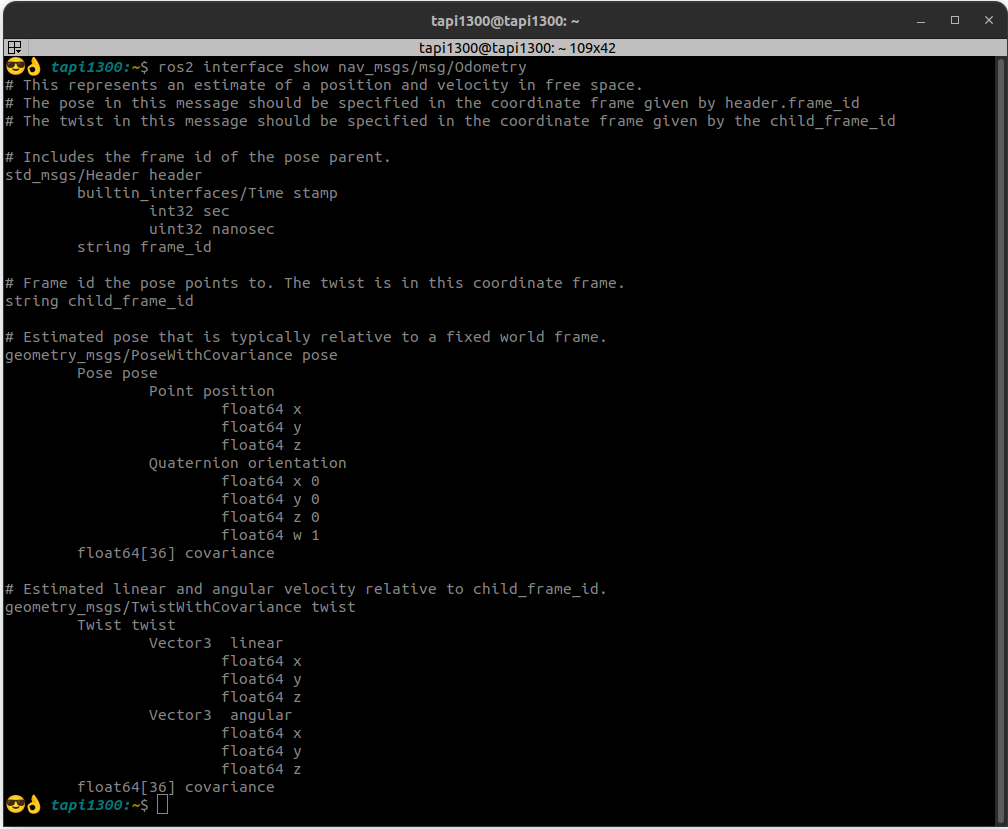
\includegraphics[width=12cm]{figs/c6/odom_msg.png}
    \end{center}
    \caption[Estructura mensaje Odometría]{Estructura del tipo de mensaje \textit{nav\_msgs/msg/Odometry}.}
    \label{fig:odom_struct}
\end{figure}

Los datos que se necesitan para la aplicación son la posición \textit{X} e \textit{Y}, al igual que la posición angular del eje \textit{Z}, por lo que esto será lo que se guarde en la
función \textit{callback} y lo que se envíe por el cable de salida usando un array formado por estos tres valores numéricos. Los primeros dos valores se pueden sacar
directamente del campo \textit{pose.pose.position} del mensaje, pero la rotación viene dada mediante cuaterniones, por lo que hay que transformarlo a ángulos de euler y obtener
el valor que se busca. Esto se realiza mediante la función \textit{Rotation} del paquete
\textit{scipy.spatial.transform}\footnote{\textbf{Librería Spicy}: \url{docs.scipy.org/doc/scipy/reference/generated/scipy.spatial.transform.Rotation.html}}
de \textit{python3}.
\begin{code}[H]
    \begin{lstlisting}[language=python]
        def callback(self, msg):
            global odom
            odom[0] = msg.pose.pose.position.x
            odom[1] = msg.pose.pose.position.y
            rot = Rotation.from_quat([msg.pose.pose.orientation.x, msg.pose.pose.orientation.y, msg.pose.pose.orientation.z, msg.pose.pose.orientation.w])
            odom[2] = rot.as_euler('xyz', degrees=True)[2]
    \end{lstlisting}
    \caption[Funciones para obtener la fuerza repulsiva]{Funciones para obtener la fuerza repulsiva.}
    \label{cod:rep_vel}
\end{code}

El siguiente bloque es el generador de destinos, que usa la ubicación del robot para comprobar si ha llegado a la actual (teniendo en cuenta un margen) y mandar
la siguiente dentro de la lista de destinos. También se ha implementado un contador de vueltas, aprovechando que se ha creado un circuito cerrado.

\begin{code}[H]
    \begin{lstlisting}[language=python]
        def main(inputs, outputs, parameters, synchronise):
            dest_arr = [[7,9],
                        [10,15],
                        [10,23],
                        [5,26],
                        [-1,23],
                        [-1,9]]
            destination = [0,0,0]
            odom = []
            first = True
            margen = 1
            actual = -1
            lap = 0
            while 1:
                odom = inputs.read_array("Odom")
                if odom is not None:
                    if(first or 
                            (odom[0] > dest_arr[actual][0]-margen and 
                            odom[0] < dest_arr[actual][0]+margen and
                            odom[1] > dest_arr[actual][1]-margen and 
                            odom[1] < dest_arr[actual][1]+margen)):
                        actual += 1
                        if(first or actual > len(dest_arr)-1):
                            lap +=1
                            actual = 0    
                            print("LAP NUMBER " + str(lap)) 
                        destination = dest_arr[actual]
                        outputs.share_array("Destination", destination)
                        print("NEW DESTINATION! " + str(destination))
                        first = False
    \end{lstlisting}
    \caption[Bloque generador de ubicaciones]{Bloque generador de ubicaciones.}
    \label{cod:dest_gen}
\end{code}

Estos dos \textit{arrays} (\textit{odom} y destino) los recibe el siguiente bloque, que es el que calcula la fuerza atractiva. Este bloque comprueba que
los datos que recibe no estén vacíos (al iniciar la ejecución puede leer \textit{null} de los cables), calculando la posición relativa del objetivo
respecto al robot tanto para los ejes \textit{X} e \textit{Y} como para la rotación relativa. En caso de que la rotación relativa supere un valor máximo,
se establece dicho máximo como valor de ángulo relativo, enviando éste como único valor, ya que en esta versión sólo se tiene en cuenta la velocidad angular,
manteniendo la lineal constante a 1 (en el VFF con máquina de estados sí se tiene en cuenta la velocidad lineal).

\begin{code}[H]
    \begin{lstlisting}[language=python]
        max_y_rel = 2
        def main(inputs, outputs, parameters, synchronise):
            while True:
                x_y_Yaw = inputs.read_array("Odom")
                dest = inputs.read_array("Destination")
                if x_y_Yaw is not None and dest is not None:
                    dx = dest[0] - x_y_Yaw[0]
                    dy = dest[1] - x_y_Yaw[1]
                    # Rotate with current angle
                    y_rel = dx * math.sin (math.radians(-x_y_Yaw[2])) + dy * math.cos (math.radians(-x_y_Yaw[2]))
                    if(y_rel > max_y_rel):
                        y_rel = max_y_rel
                    elif(y_rel < -max_y_rel):
                        y_rel = -max_y_rel
                    outputs.share_number("AttrForce", y_rel)
    \end{lstlisting}
    \caption[Bloque fuerza atractiva]{Bloque que calcula la fuerza atractiva.}
    \label{cod:attr_vel}
\end{code}

Por último, ambas fuerzas se combinan en un mismo bloque, que es el encargado de sumar ambas fuerzas y transformarlas en velocidad angular. Para ello aplica
un valor a modo de controlador constante para que la fuerza repulsiva sea más significativa que la atractiva y permitir que el robot esquive objetos que
puedan quedar muy cercanos. Finalmente se envía el \textit{array} de velocidades manteniendo la velocidad lineal a 1 y siendo la velocidad angular el valor
calculado por el algoritmo.

\begin{code}[H]
    \begin{lstlisting}[language=python]
        import math

        def main(inputs, outputs, parameters, synchronise):
            maximo = 3
            while True:            
                rep = inputs.read_number("RepForce")
                attr = inputs.read_number("AttrForce")
                if rep is not None and attr is not None:
                    final_w = 1.4*rep + 0.4*attr
                    if(final_w > maximo):
                        final_w = maximo
                    elif(final_w < -maximo):
                        final_w = -maximo
                    outputs.share_array("Vels", [1,0,0,0,0,final_w])
    \end{lstlisting}
    \caption[Bloque fuerzas a velocidades]{Bloque que transforma las fuerzas en velocidades.}
    \label{cod:VFF_force_to_vel}
\end{code}

\subsection{Validación experimental}
\label{subsec:val_exp_VFF}
Para comprobar que el algoritmo funcionase, se han realizado varias pruebas: sólo fuerza repulsiva con obstáculos y sin ellos, y el algoritmo completo con un
bloque de depuración (\ref{subsec:spec_bloques_FSM}).

Para las primeras pruebas el circuito contaría únicamente con 3 bloques: el bloque del sensor láser, el que calcula la fuerza repulsiva y el bloque MotorDriverROS2:

\begin{figure} [H]
    \begin{center}
        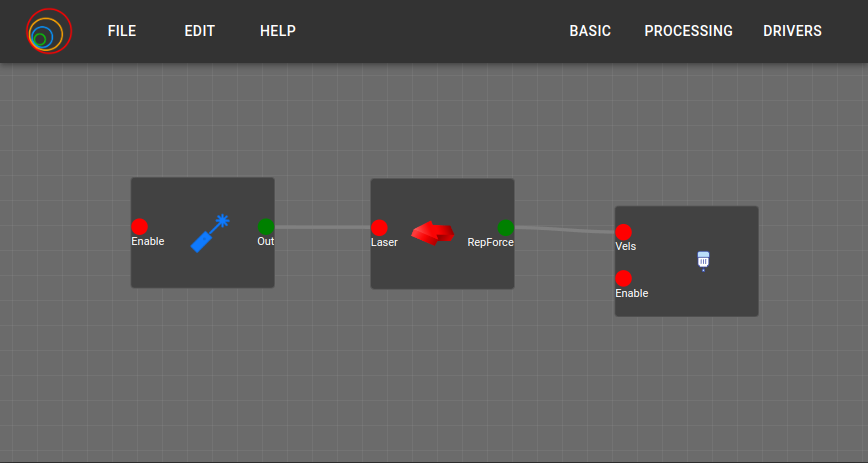
\includegraphics[width=9cm]{figs/c6/VFF_r_Circ.png}
    \end{center}
    \caption[Circuito VFF sólo fuerza repulsiva]{Circuito de VFF sólo con la fuerza repulsiva.}
    \label{fig:VFF_r_circ}
\end{figure}

Como podemos comprobar en las siguientes secuencias y en sus vídeos correspondientes, la parte de la fuerza repulsiva cumple con el objetivo, ya que mantiene
al robot alejado de las paredes del circuito a la vez que evita los obstáculos (en el caso en el que los hay).

\begin{figure} [H]
    \begin{center}
        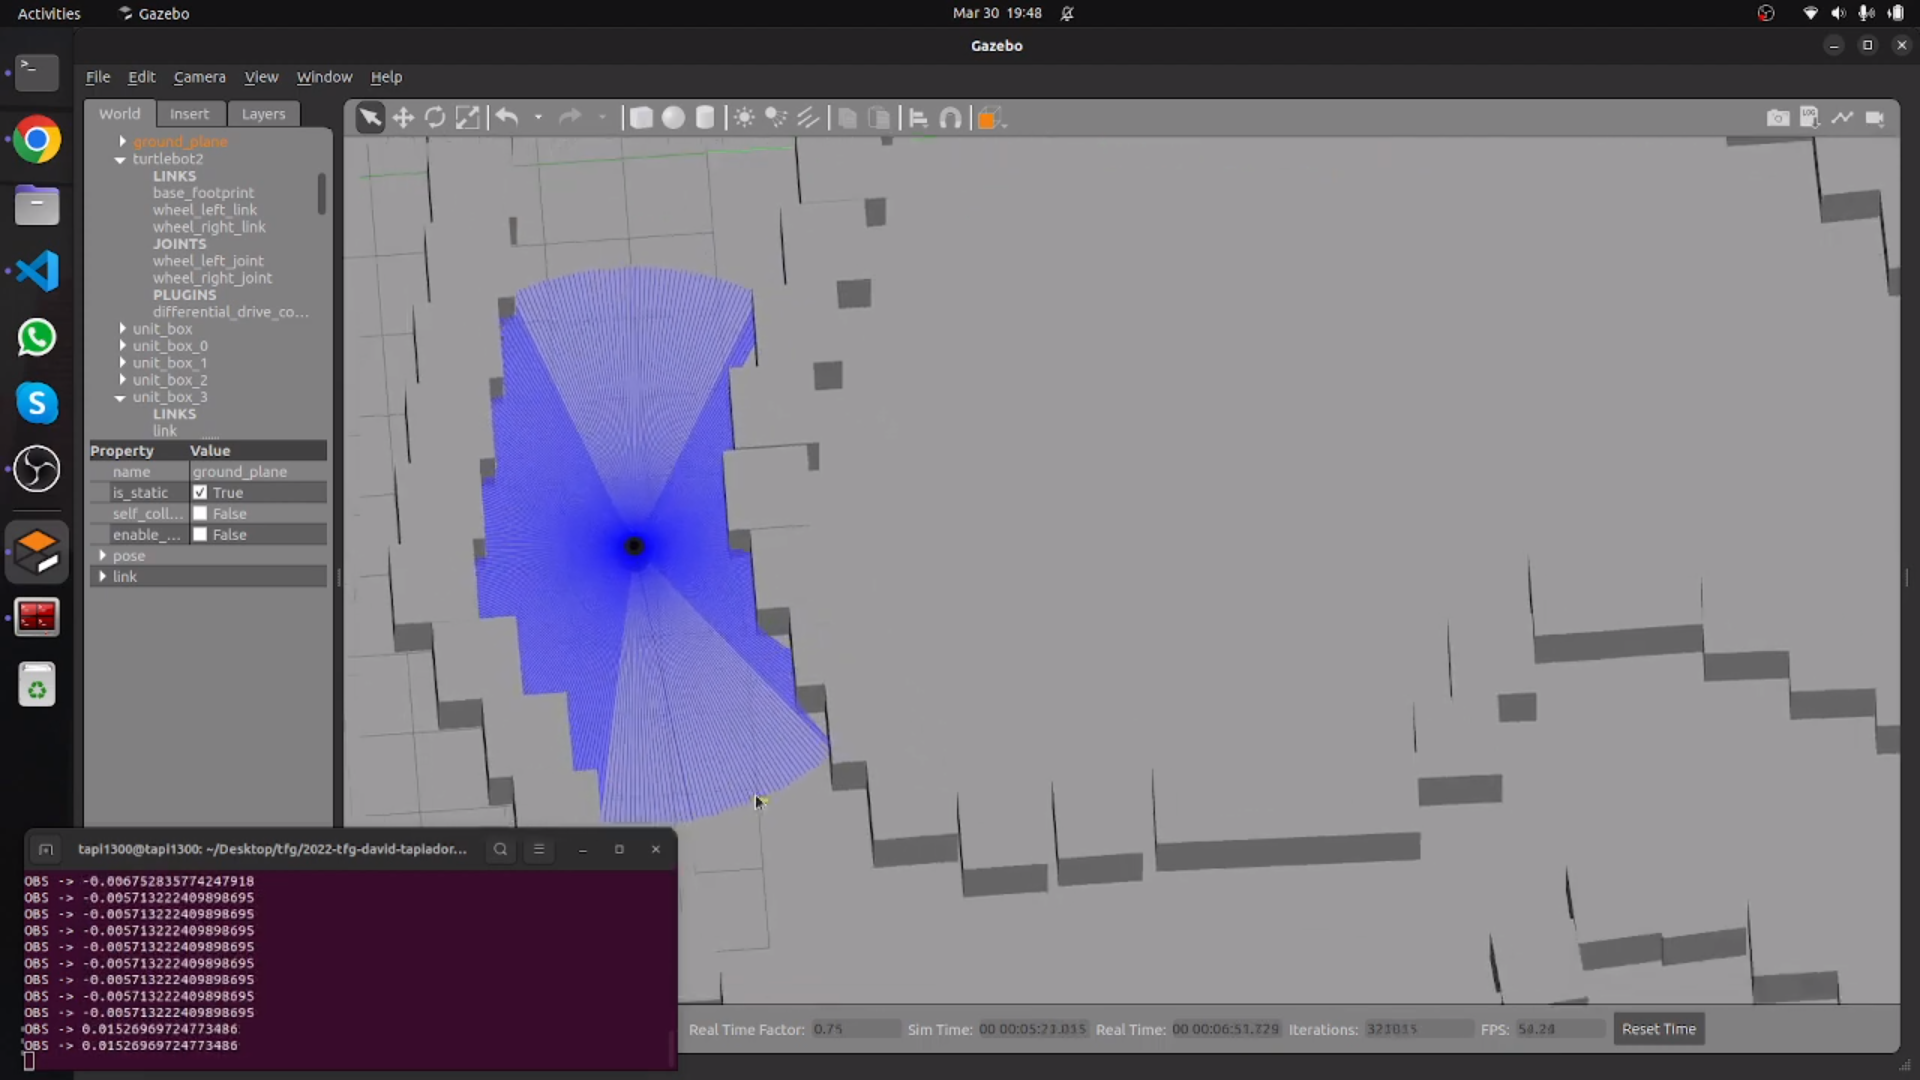
\includegraphics[width=7cm]{figs/c6/VFF_rs1.png}
        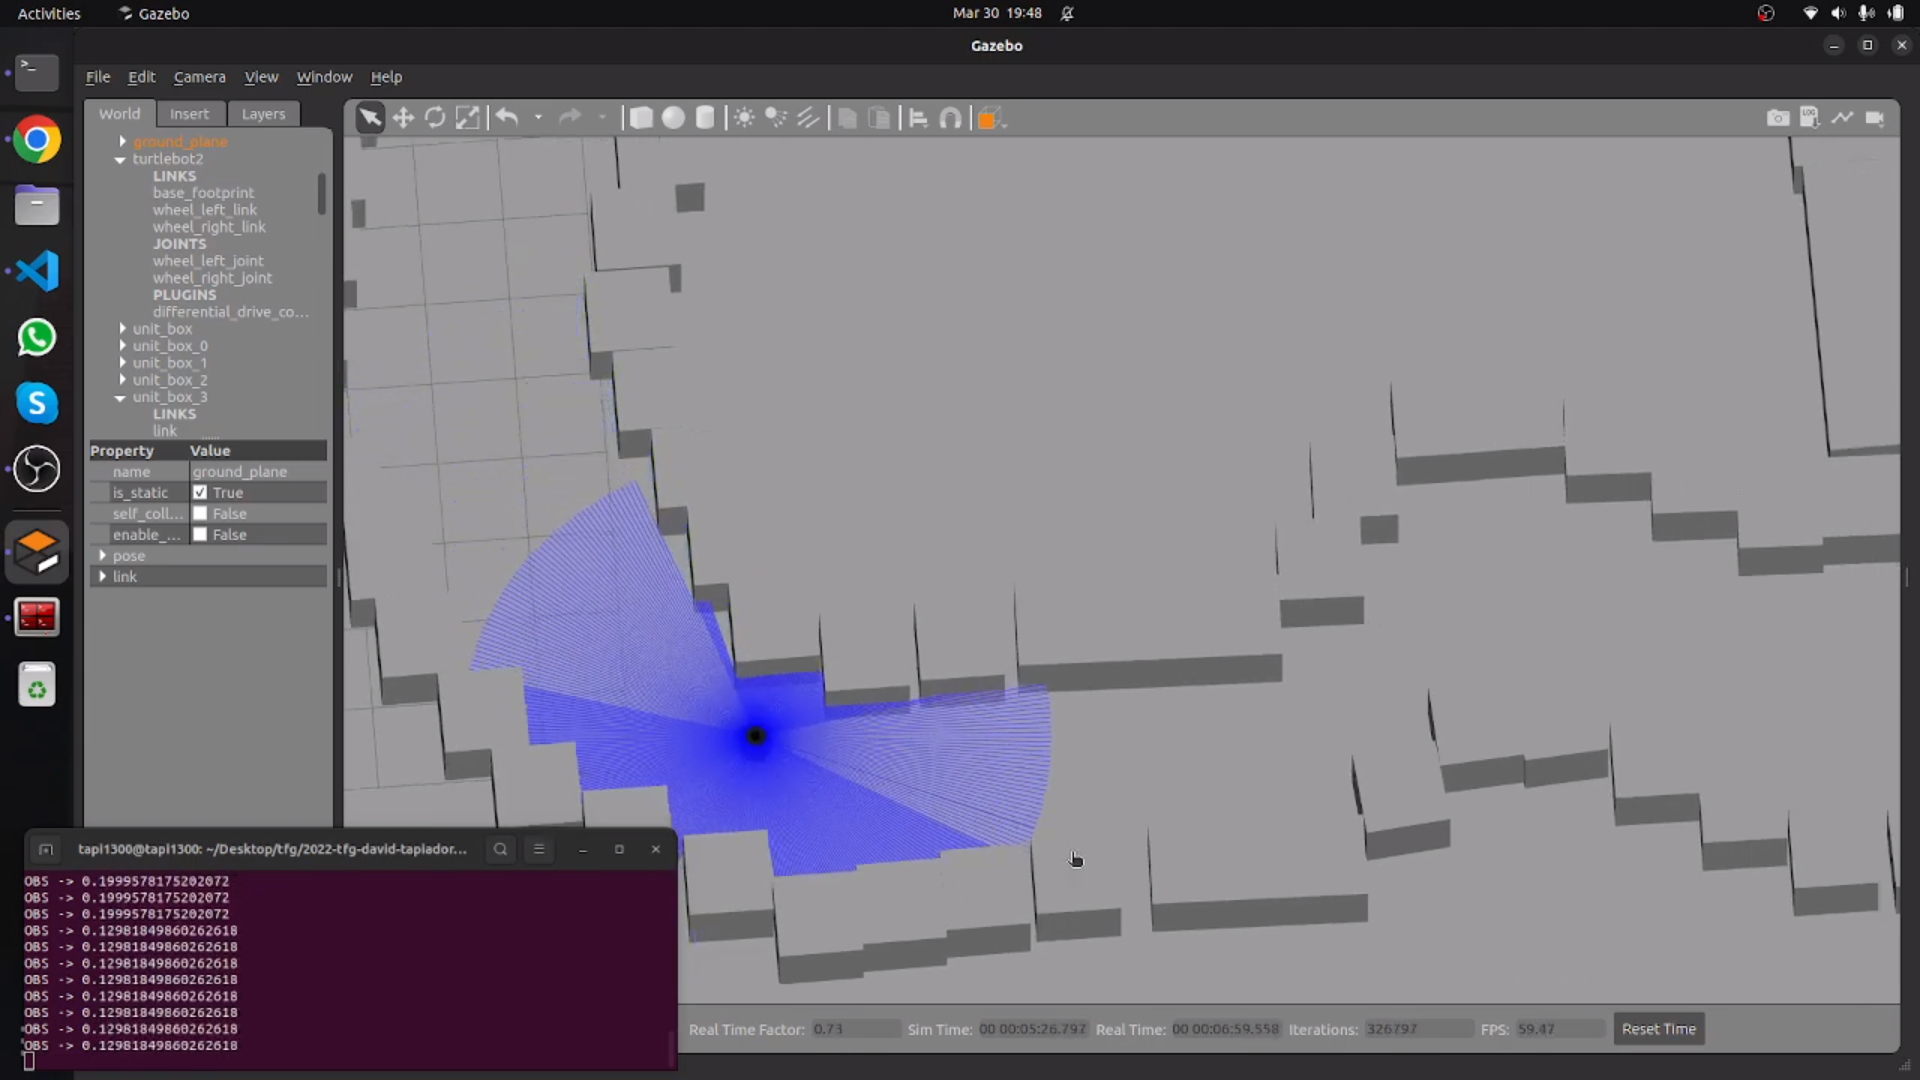
\includegraphics[width=7cm]{figs/c6/VFF_rs2.png}
    \end{center}
    \caption[Secuencia VFF fuerza repulsiva sin obstáculos]{VFF usando sólo la fuerza repulsiva sin obstáculos. Imagenes obtenidas de Youtube\footnotemark.}
    \label{fig:VFF_r_S}
\end{figure}
\footnotetext{\textbf{Vídeo VFF fuerza repulsiva sin obstáculos}: \url{https://www.youtube.com/watch?v=uhtBRw96Zl4&ab_channel=Tapii}}
\begin{figure} [H]
    \begin{center}
        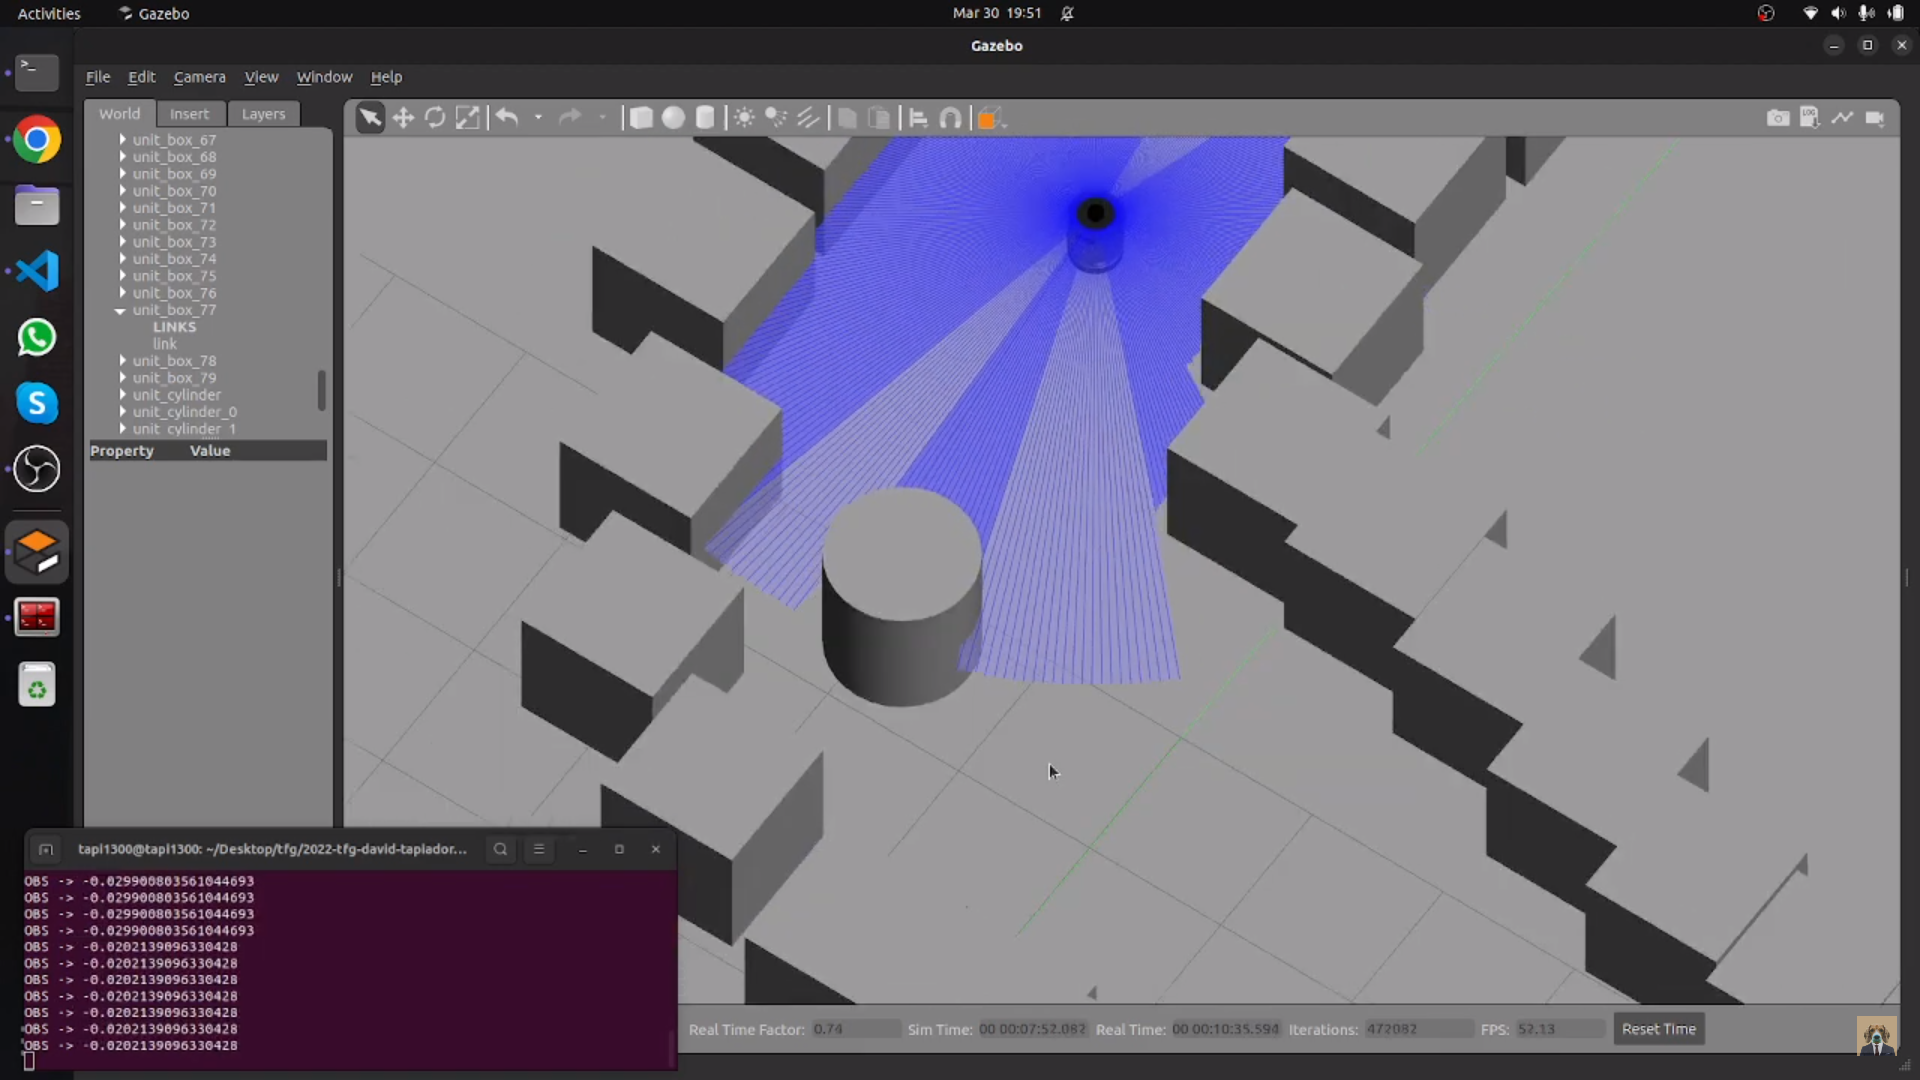
\includegraphics[width=7cm]{figs/c6/VFF_rc1.png}
        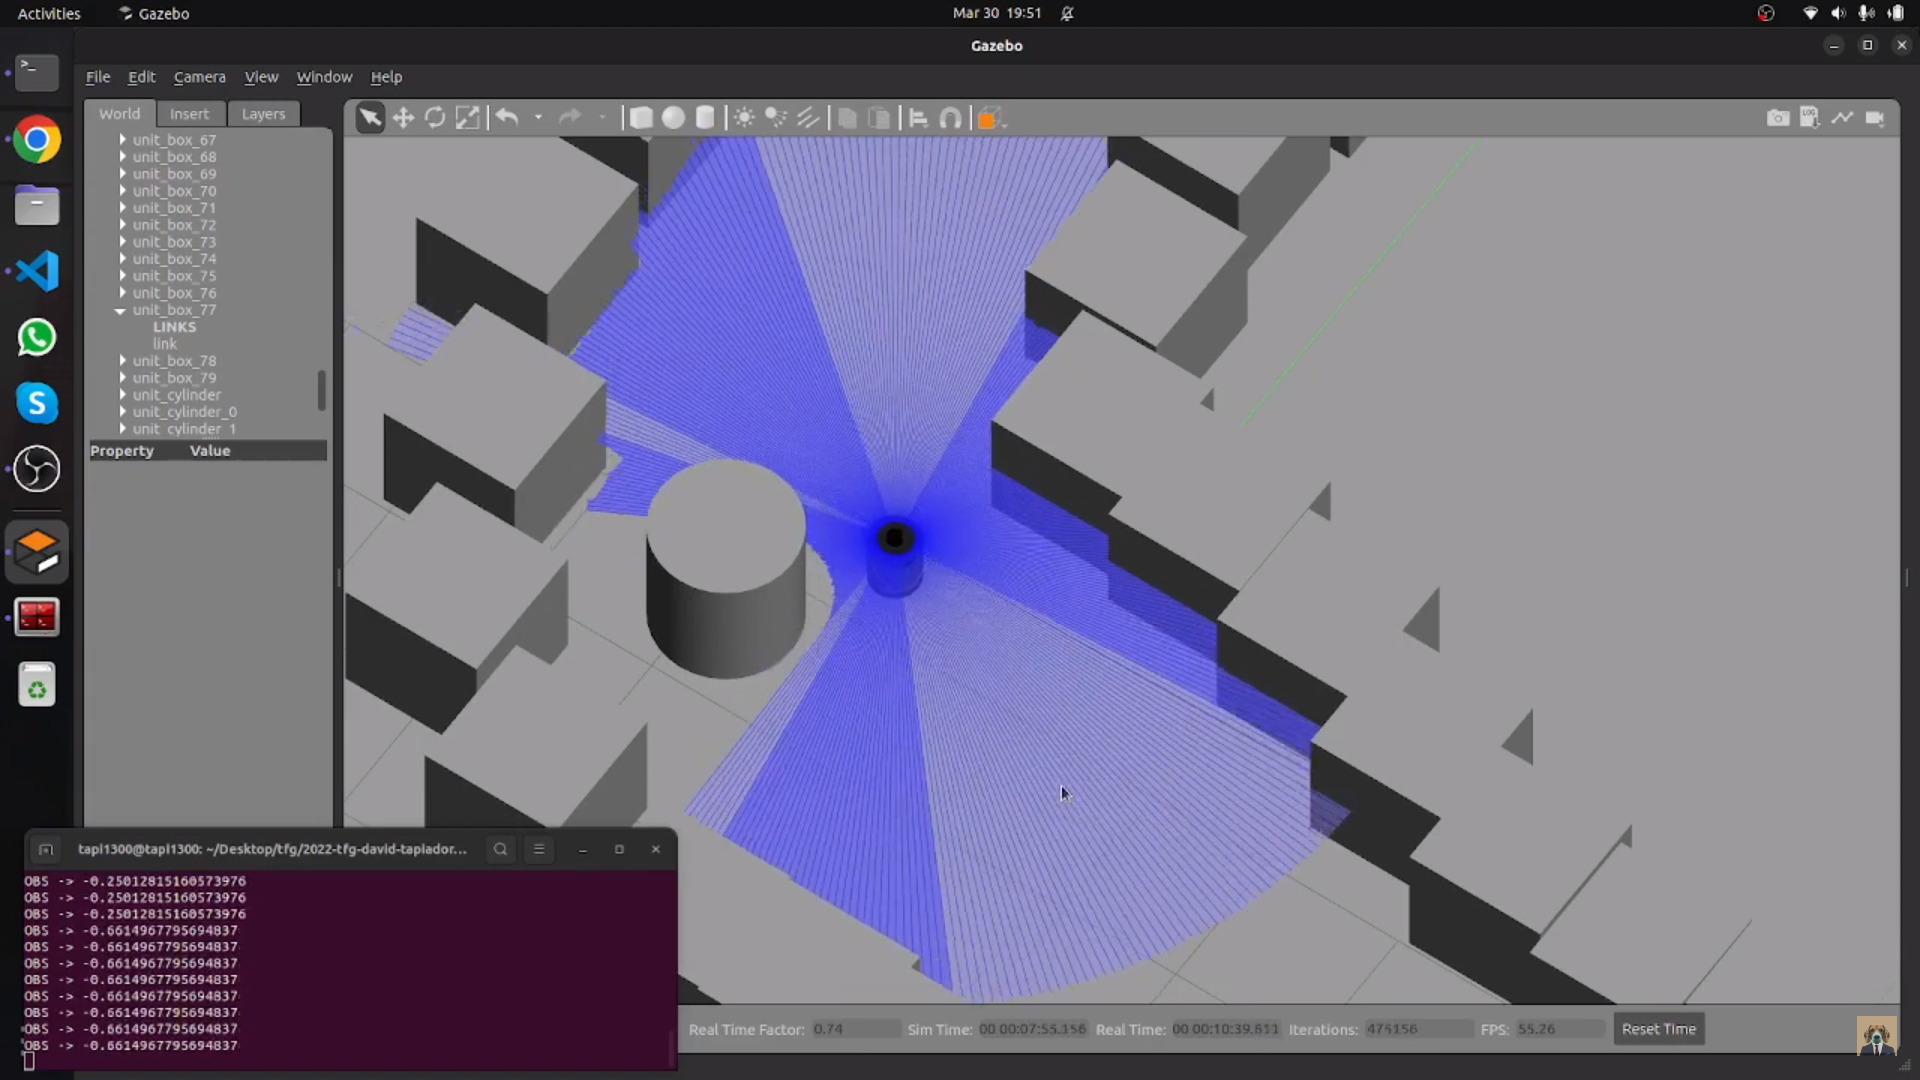
\includegraphics[width=7cm]{figs/c6/VFF_rc2.png}
    \end{center}
    \caption[Secuencia bloque MotorDriverROS2 real]{VFF usando sólo la fuerza repulsiva con obstáculos. Imagenes obtenidas de Youtube\footnotemark.}
    \label{fig:MotordriverReal}
\end{figure}
\footnotetext{\textbf{Vídeo VFF fuerza repulsiva con obstáculos}: \url{https://www.youtube.com/watch?v=HeTFum_gTGw&ab_channel=Tapii}}

En la siguiente prueba, el circuito usado incluye el bloque display (se describirá su funcionamiento en el siguiente punto, ya que aquí no estaba completamente
desarrollado) y un bloque \textit{screen} para mostrar la imagen de este bloque.

\begin{figure} [H]
    \begin{center}
        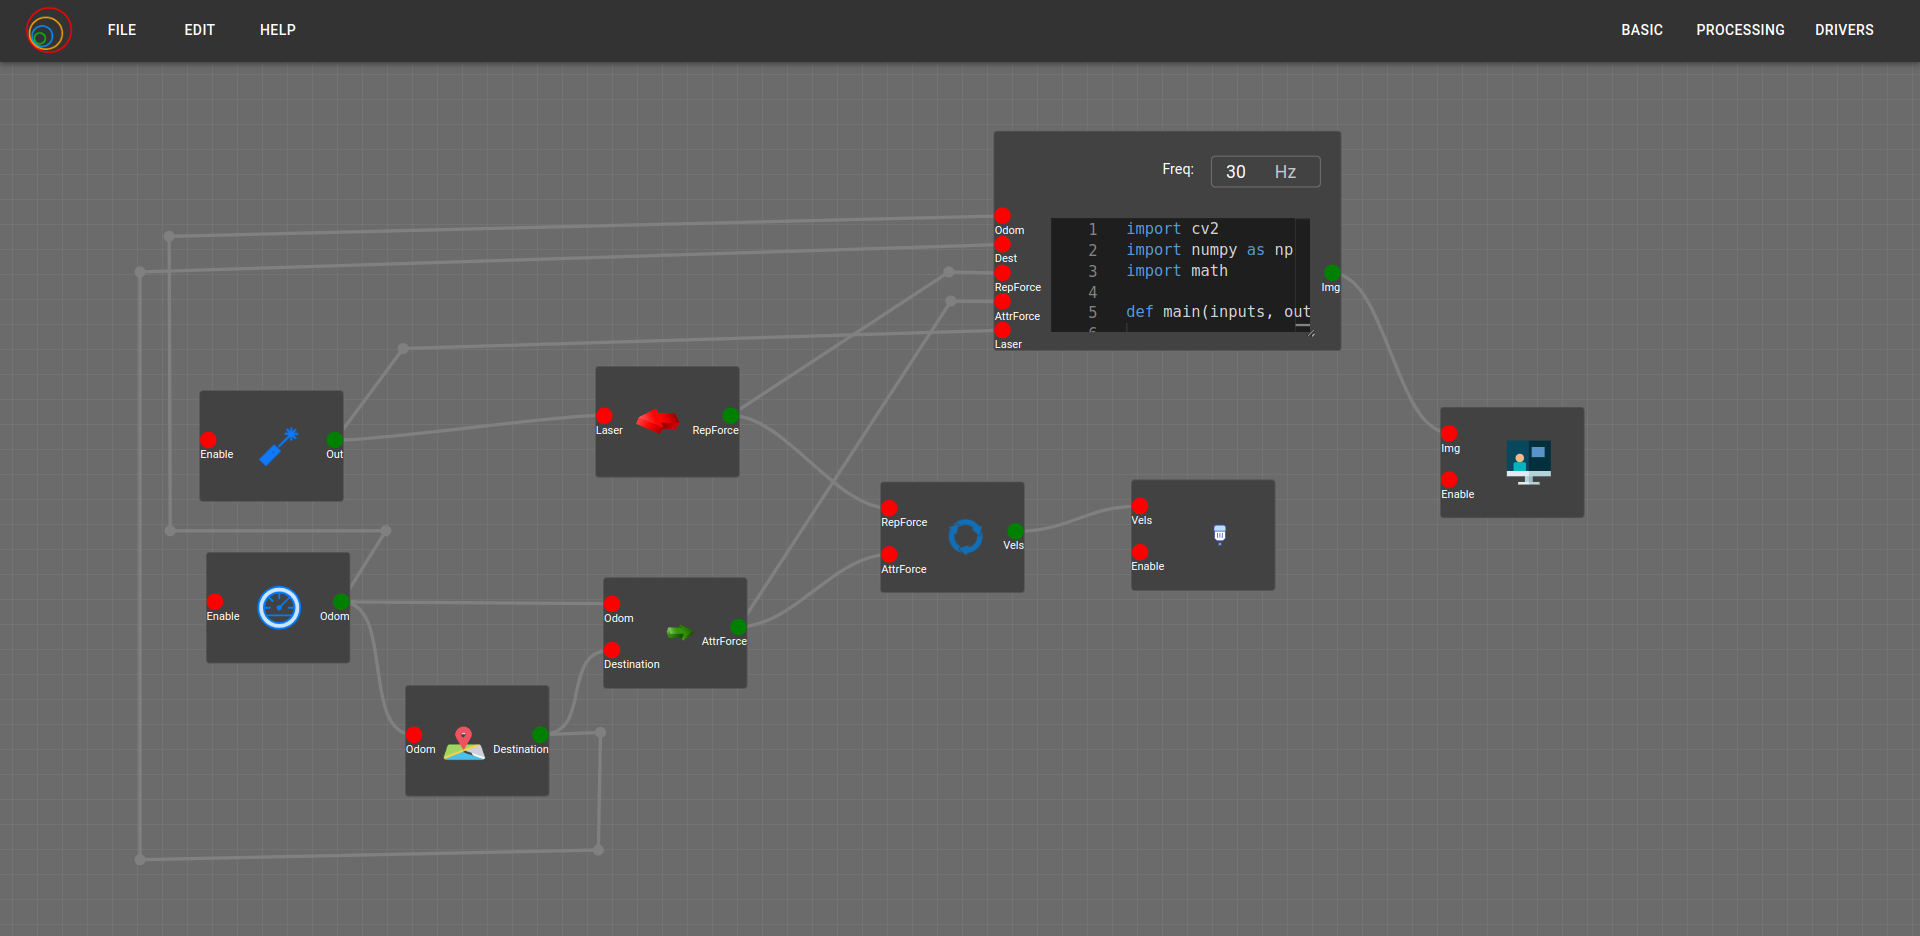
\includegraphics[width=10cm]{figs/c6/VFF_disp_circ.png}
    \end{center}
    \caption[Circuito VFF]{Circuito del algoritmo VFF.}
    \label{fig:VFF_disp_circ}
\end{figure}

\begin{figure} [H]
    \begin{center}
        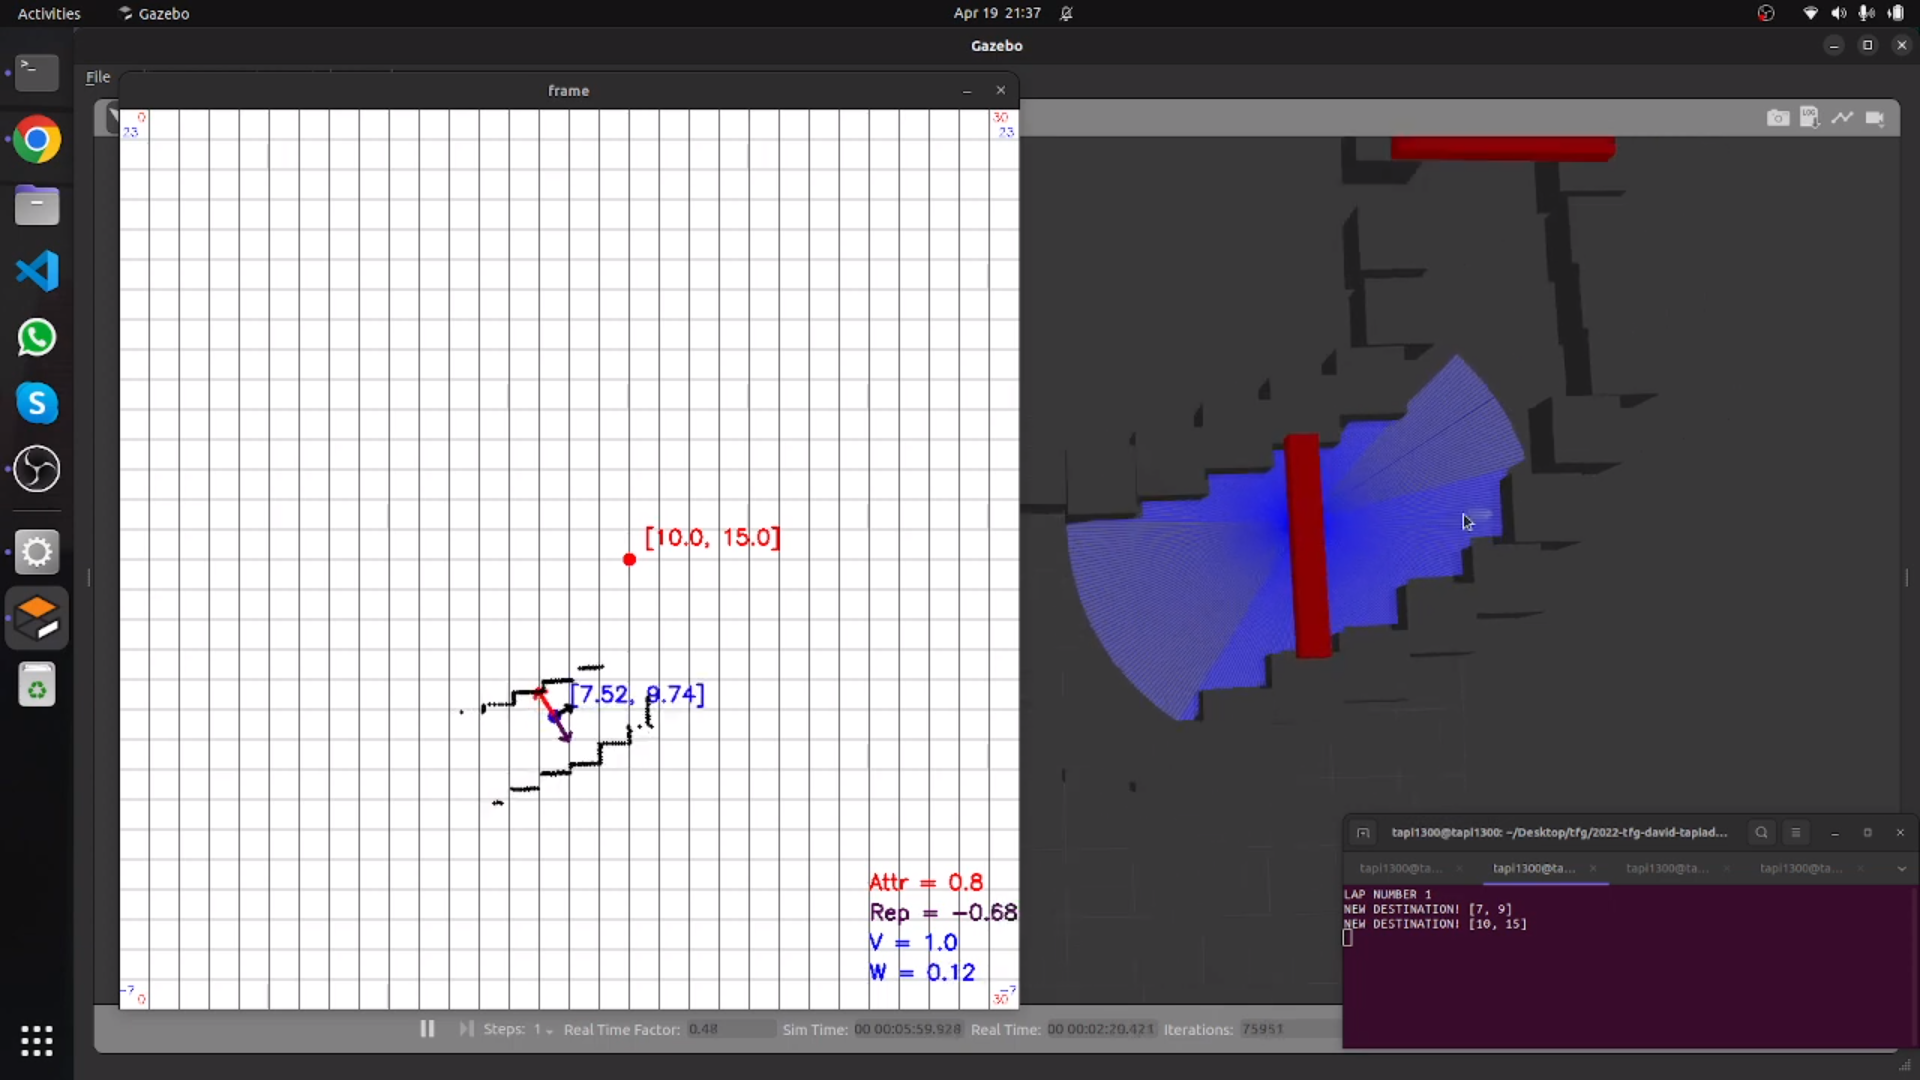
\includegraphics[width=7cm]{figs/c6/VFF_d1.png}
        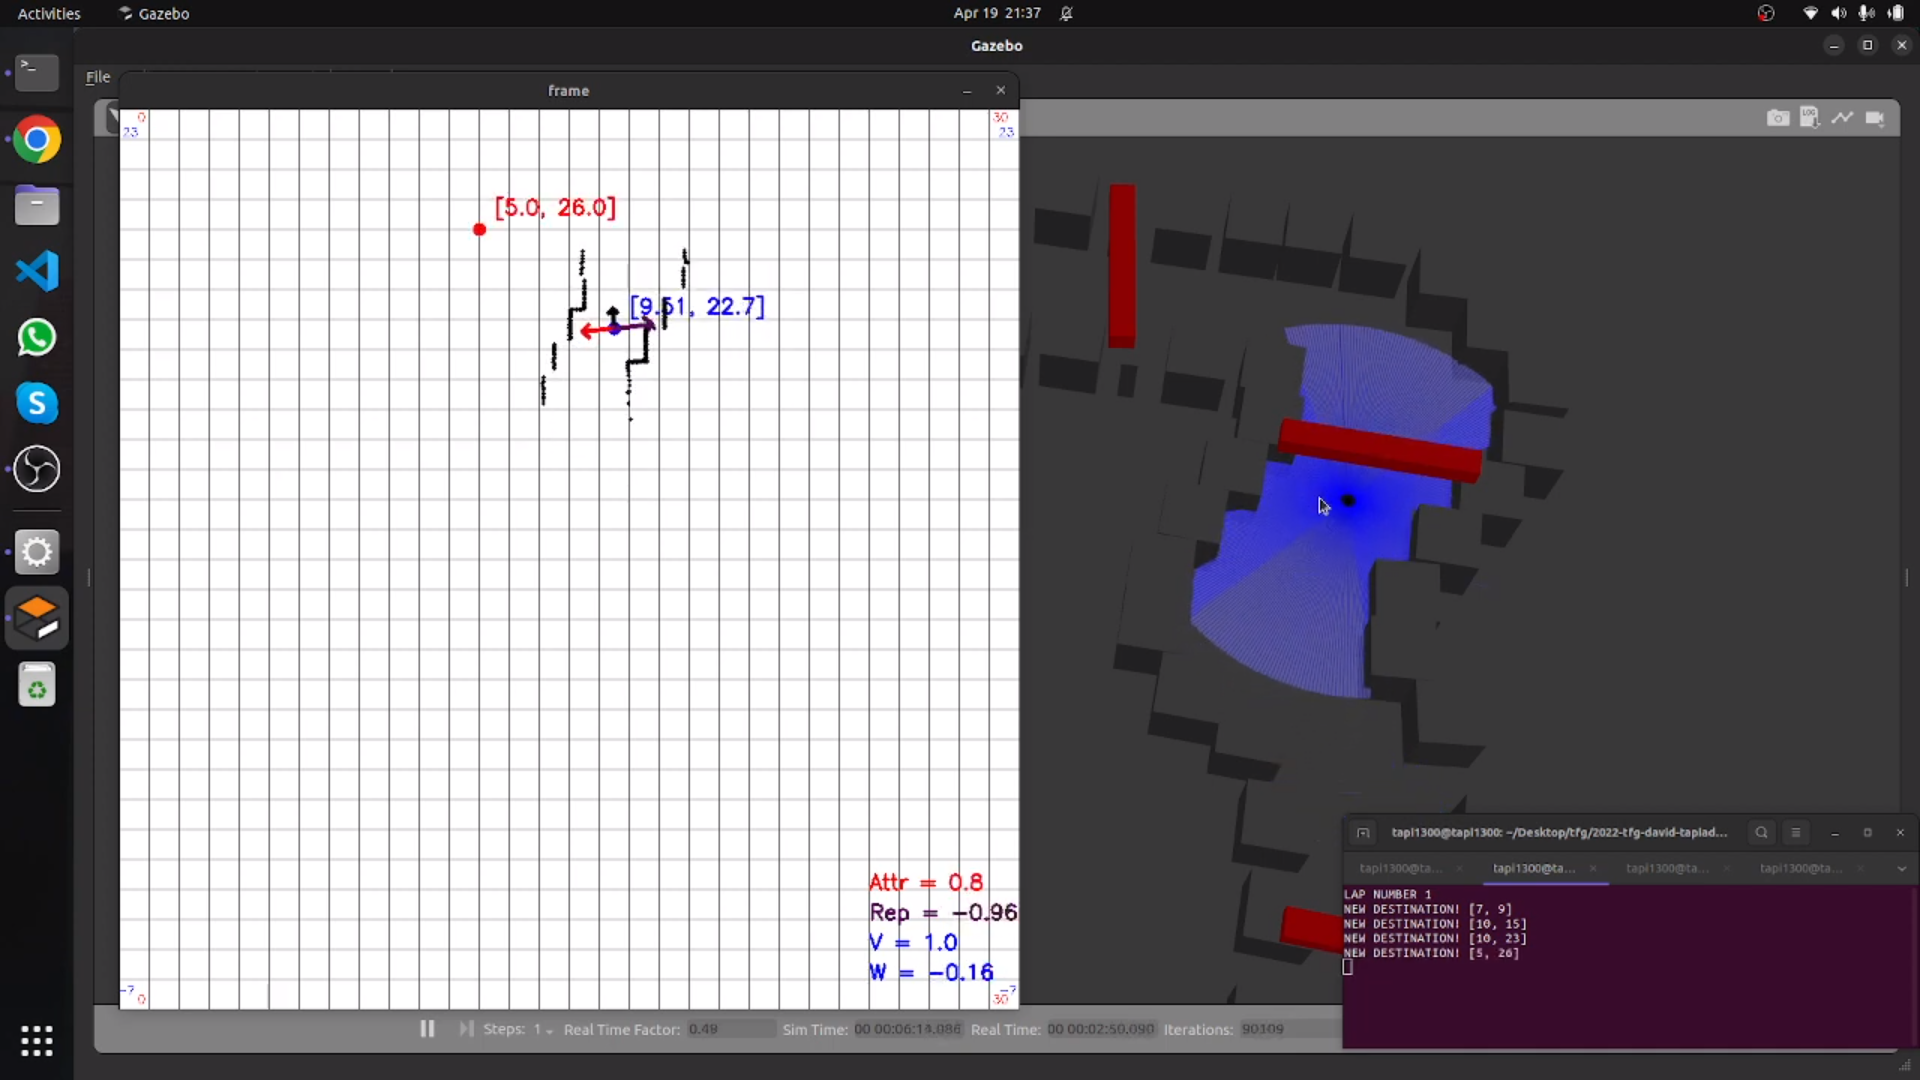
\includegraphics[width=7cm]{figs/c6/VFF_d2.png}
    \end{center}
    \caption[Secuencia prueba VFF]{Secuencia de pruebas del algoritmo VFF. Imagenes obtenidas de Youtube\footnotemark.}
    \label{fig:VFF_pruebas}
\end{figure}
\footnotetext{\textbf{Vídeo VFF con display}: \url{https://www.youtube.com/watch?v=xdGCIrYFu7E&t=108s&ab_channel=Tapii}}

\section{VFF mediante máquina de estados}
\label{sec:FSM}

Una vez que el algoritmo está practicamente desarrollado, se va a implementar una máquina de estados. Esta máquina de estados tendrá 3 estados distintos: generar ubicación
aleatoria, ir a la ubicación y volver al punto de salida (después de varias ubicaciones aleatorias).\\

Como se puede ver en el siguiente diagrama, la ejecución se inicia
generando una ubicación aleatoria que se envía al estado VFF. Cuando se ha ido a 4 ubicaciones aleatorias, se pasa al estado "\textit{Return Home}", que envía la ubicación
inicial del robot como nuevo destino para el estado VFF. Una vez que llegue al inicio, se detiene al robot.

\begin{figure} [H]
    \begin{center}
        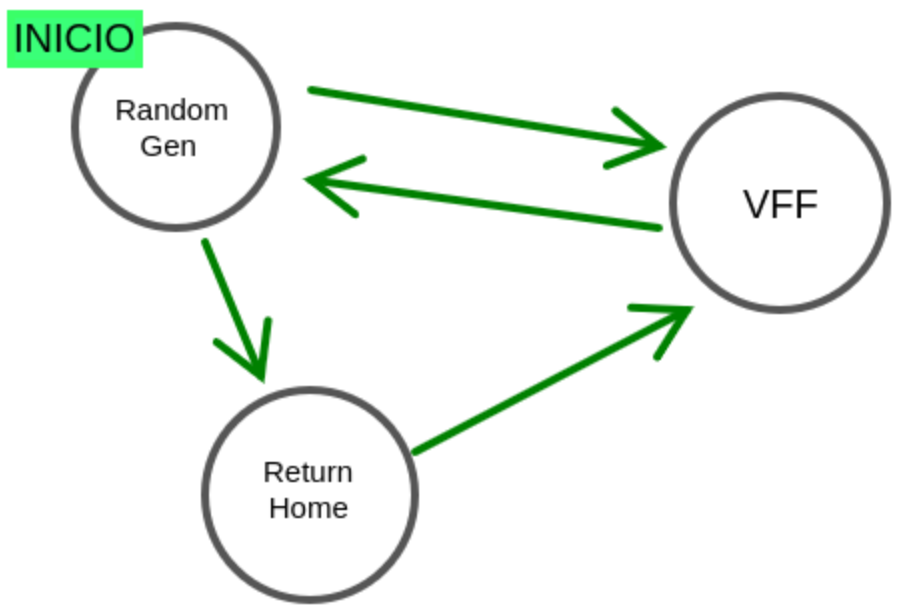
\includegraphics[width=10cm]{figs/c6/FSM_diag.png}
    \end{center}
    \caption[Diagrama máquina de estados]{Diagrama de la máquinas de estados.}
    \label{fig:FSM_diag}
\end{figure}

\subsection{Diseño del circuito y escenario}
\label{subsec:dis_bloques_FSM}

Para implementar el comportamiento de máquina de estados, se han implementado dos bloques nuevos para los comportamientos nuevos. También se ha colocado el bloque de la odometría
como un sensor general, ya que se usa en varios estados, mientras que el estado VFF está separado visualmente para que sea más sencillo de reconocer.

\begin{figure} [H]
    \begin{center}
        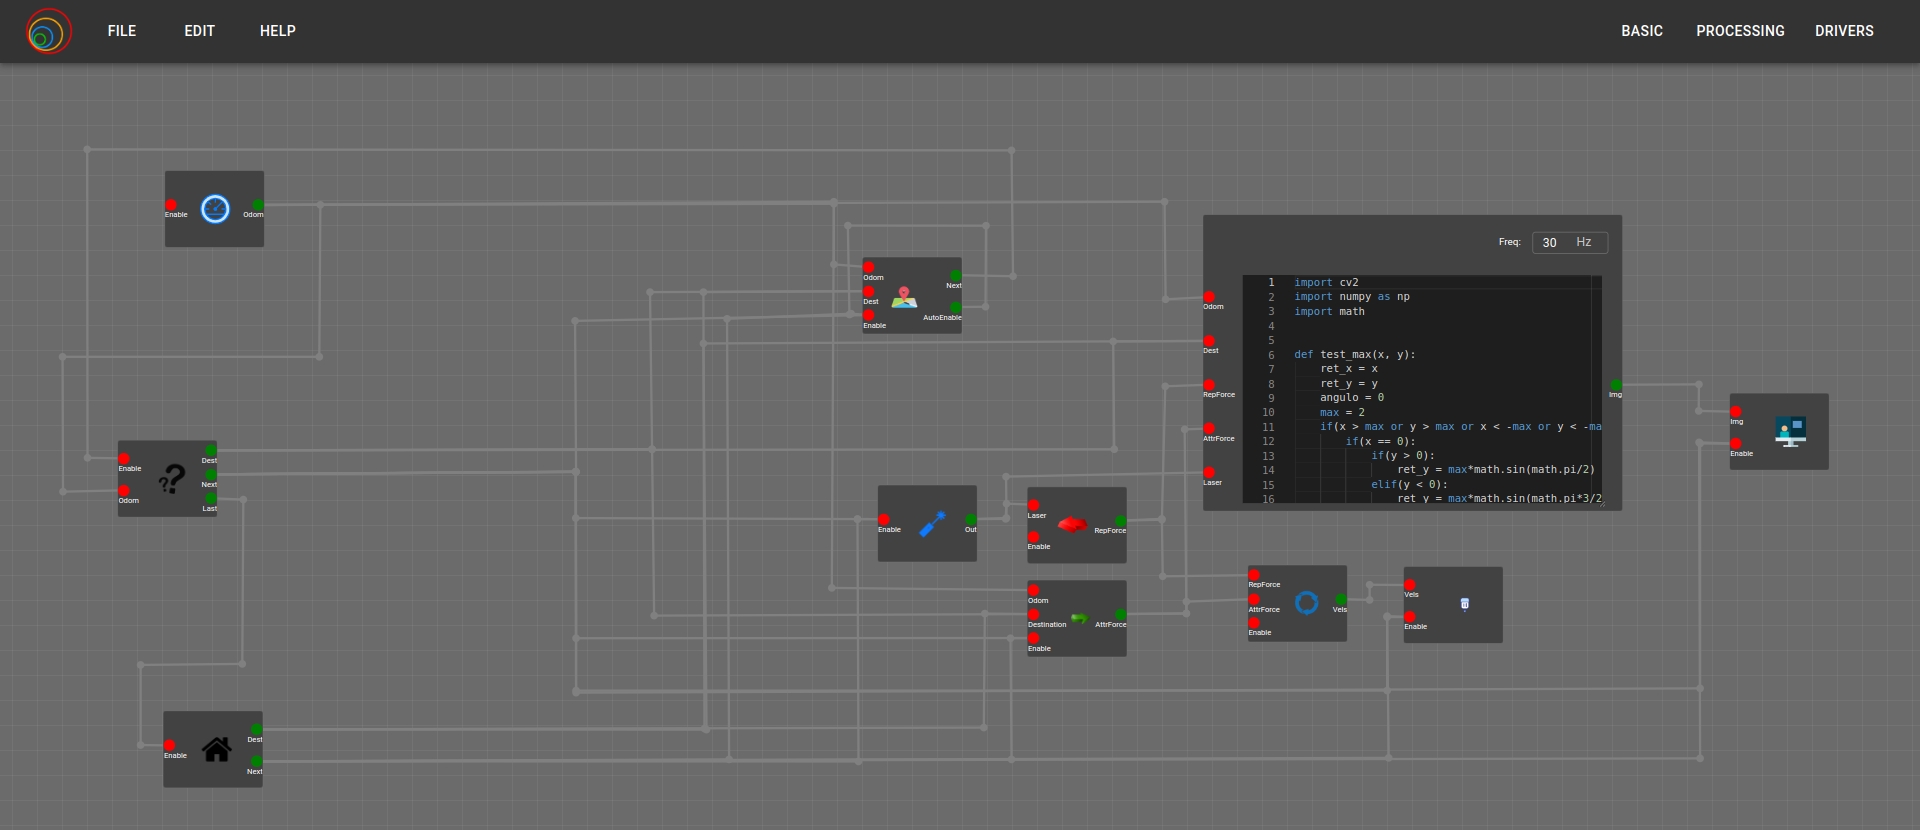
\includegraphics[width=13cm]{figs/c6/FSM_circuit.png}
    \end{center}
    \caption[Circuito VFF con FSM]{Circuito de VFF usando máquinas de estados.}
    \label{fig:FSM_circ}
\end{figure}

Como los objetivos ahora son aleatorios, no se puede usar el circuito que teníamos en el apartado anterior, por lo que se ha creado un mundo en el que se han
repartido varios cilindros por todo el mapa para que el robot tenga que moverse hasta el objetivo esquivándolos.

\begin{figure} [H]
    \begin{center}
        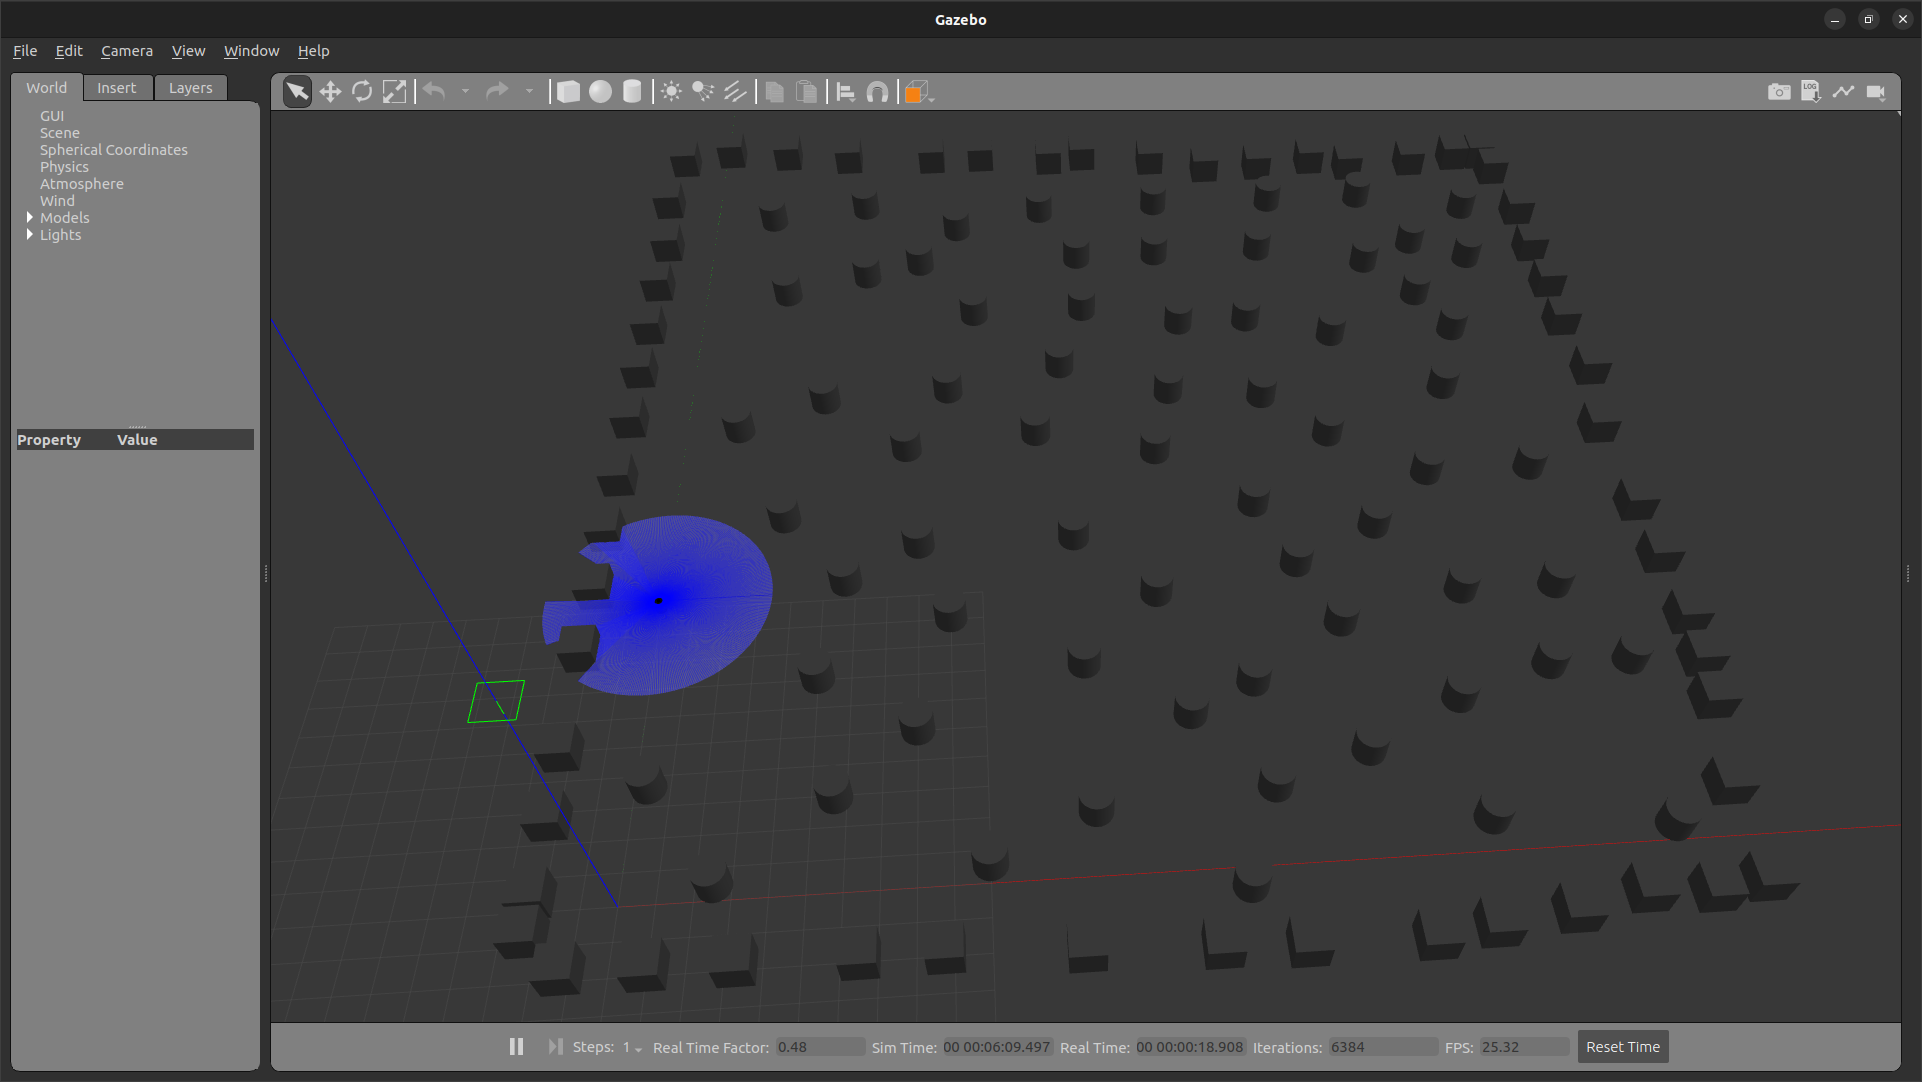
\includegraphics[width=13cm]{figs/c6/FSM_world.png}
    \end{center}
    \caption[Mundo VFF con FSM]{Mundo para probar el VFF con máquinas de estados.}
    \label{fig:FSM_world}
\end{figure}

\subsection{Bloques específicos}
\label{subsec:spec_bloques_FSM}

Para ampliar el funcionamiento del VFF para que también tenga en cuenta las fuerzas para calcular la velocidad lineal, se ha tenido que modificar los bloques que calculan las
fuerzas atractiva y repulsiva (\ref{cod:parse_laser_data} y \ref{cod:attr_vel}), por lo que en vez de mandar una única fuerza, se mandan la fuerza como vector (componente X e Y).
También se han añadido lecturas al \textit{input enable}, ya que es el que habilita activar y desactivar los bloques, únicamente ejecutando los bloques que estén activos en ese
momento y manteniendo el resto en estado inactivo.

\begin{code}[H]
    \begin{lstlisting}[language=python]
        # Cambio en bloque de fuerza repulsiva
        outputs.share_array("RepForce", [obsX/50, obsY/50])

        # Cambio en bloque de fuerza atractiva
        outputs.share_array("AttrForce", [x_rel, y_rel])

        # Bucle principal bloque laser
        while 1:
            enable = inputs.read_number('Enable')
            if enable == 1:
                measure = None
                rclpy.spin_once(laser_subscriber)
                if measure is not None:
                    outputs.share_array("Out",measure)  
    \end{lstlisting}
\end{code}

Uno de los bloques nuevos es el generador de ubicaciones aleatorias. Éste también es el que se encarga de decidir cuál será el siguiente estado. Para ello tiene un contador
interno que le permite saber cuántas veces se han generado ubicaciones aleatorias y, cuando se llegue al valor de \textit{max\_times} se cambia al estado de volver al origen.
Para generar la ubicación aleatoria, generamos un número que cumpla que num1 esté entre \textit{x-márgen} y \textit{x+márgen} y otro num2 que esté entre \textit{y-márgen} y \textit{y+márgen},
para evitar ubicaciones que estén demasiado alejadas del robot. También dicho número debe estar entre 0 y 30, ya que estos son los límites del mundo (máximo que se
representa dentro del bloque \textit{display}).

\begin{code}[H]
    \begin{lstlisting}[language=python]
    from random import randint
    import time

    def main(inputs, outputs, parameters, synchronise):
        first = True
        changed = False
        times = 0
        max_times = 4
        margen = 3
        x = [0,30]
        y = [0,30]
        while 1:    
                enable = inputs.read_number("Enable")
                if(enable == 0):
                    changed = False
    \end{lstlisting}
\end{code}
\begin{code}[H]
    \begin{lstlisting}[language=python]
                if (enable == 1 or first) and not changed:
                    odom = inputs.read_array("Odom")
                    if odom[0] != None:
                        changed = True
                        first = False
                        times += 1
                        if(times < max_times):
                            print("***ESTADO ACTIVADO -> GENERAR UBICACION ALEATORIA***")
                            dest = [randint(x[0]+1, x[1]-1),
                                        randint(y[0]+1,y[1]-1)]

                            while dest[0] > int(odom[0]-margen) and dest[0] < int(odom[0]+margen):
                                dest[0] = randint(x[0]+1, x[1]-1)
                            while dest[1] > int(odom[1]-margen) and dest[1] < int(odom[1]+margen):
                                dest[1] = randint(y[0]+1,y[1]-1)
                                
                            print("NUEVO DESTINO -> " + str(dest))
                            time.sleep(2)
                            print("***ESTADO ACTIVADO -> VFF***")
                            outputs.share_array("Dest", dest)
                            outputs.share_number("Next", 1)
                            outputs.share_number("Last", 0)
                        else:
                            print("***ESTADO ACTIVADO -> VUELTA AL ORIGEN***")
                            outputs.share_number("Next", 0)
                            outputs.share_number("Last", 1)
    \end{lstlisting}
    \caption[Bloque generador aleatorio de destinos]{Bloque que genera destinos aleatorios y decide el siguiente estado.}
    \label{cod:FSM_asker}
\end{code}

El siguiente bloque nuevo es el correspondiente al estado de volver al inicio. Cuando este bloque se activa, envía la ubicación del origen al estado VFF e imprime
varias trazas para saber en qué punto del comportamiento se encuentra la ejecución.

\begin{code}[H]
    \begin{lstlisting}[language=python]
        import time
        def main(inputs, outputs, parameters, synchronise):
            dest = [2,10]
            first = True
            going = False
            while 1:
                enable = inputs.read_number("Enable")
                if enable == 1 and first:
                        print("UBICACION DEL ORIGEN -> " + str(dest))
                        time.sleep(2)
                        outputs.share_array("Dest", dest)
                        outputs.share_number("Next", 1)
                        first = False
                if enable == 0 and not first:
                    going = True
                if enable == 1 and going:
                    print("HEMOS LLEGADO AL ORIGEN!!")
                    outputs.share_number("Next", 0)
    \end{lstlisting}
    \caption[Bloque return home]{Bloque para volver al inicio.}
    \label{cod:FSM_return_home}
\end{code}

El bloque que transforma las fuerzas a velocidades también cambia, ya que ahora hay que tener en cuenta la componente lineal de las fuerzas y, por lo tanto, calcular nuevas
proporciones y evaluar valores máximos y mínimos. También se ha añadido que, si la velocidad lineal es negativa y la angular es cercana a 0 (valor absoluto menor que 0.3), se
ponga al robot a girar estático. Esto es para evitar objetivos que se encuentren detrás del robot y que, por lo tanto, intente llegar a ellos marcha atrás.

\begin{code}[H]
    \begin{lstlisting}[language=python]
        def main(inputs, outputs, parameters, synchronise):
            max_v = 2
            min_v = 0.5
            max_w = 3
            alpha_V = 1
            beta_V = 1
            alpha_W = 0.7
            beta_W = 1.4
            while 1:
                rep = inputs.read_array("RepForce")
                attr = inputs.read_array("AttrForce")
                if rep is not None and attr is not None:
                    attr_x, attr_y = test_max(attr[0],attr[1])
                    rep_x, rep_y = test_max(rep[0],rep[1])
                    final_v = alpha_V*attr_x + beta_V*rep_x
                    final_w = alpha_W*attr_y + beta_W*rep_y
    \end{lstlisting}
\end{code}
\begin{code}[H]
    \begin{lstlisting}[language=python]
                    if(final_v < 0 and final_w < 0.3 and final_w > 0.3):
                        # Rotar en el sitio hasta que no sea sentido opuesto
                        final_v = 0
                        final_w = max_w/3
                    elif(final_v > max_v):
                        final_v = max_v
                    elif(final_v < min_v):
                        final_v = min_v

                    if(final_w > max_w):
                        final_w = max_w
                    elif(final_w < -max_w):
                        final_w = -max_w

                    outputs.share_array("Vels", [final_v,0,0,0,0,final_w])
    \end{lstlisting}
    \caption[Bloque forces to vels]{Bloque que pasa de fuerzas a velocidades.}
    \label{cod:FSM_forcestovels}
\end{code}

Por último, el bloque \textit{display} consiste en crear una imagen mediante un \textit{array} de \textit{numpy} en el que se muestra aproximadamente una representación del
mundo que ve el robot. Aquí se muestran tanto la ubicación del robot y del destino, como las fuerzas atractiva (verde), repulsiva (roja) y total (naranja), sus valores y las lecturas
del láser mediante pequeños puntos. También se ha representado cada metro cuadrado del simulador mediante una cuadrícula en la imagen.

Aquí se usa la librería cv2 de opencv-python\footnote{\textbf{OpenCV-Python}: \url{https://pypi.org/project/opencv-python/}} para editar la imágen, para insertar
líneas (\textit{cv2.line} para líneas y \textit{cv2.arrowedLine} para flechas) y para escribir texto (\textit{cv2.putText}), al igual que la librería \textit{math}
(\textit{cos}, \textit{sin}, \textit{radians}, \textit{sqrt}, ...) para calcular la orientación de las flechas de las distintas fuerzas.

Dada la extensión del código, no se va a incluir en esta memoria, por lo que
aquí\footnote{\textbf{Código bloque display}: \url{https://github.com/RoboticsLabURJC/2022-tfg-david-tapiador/blob/main/FSM/ZIPS/FSM_final/modules/Code_1.py}}
se puede acceder a él.

\subsection{Validación experimental}
\label{subsec:val_exp_FSM}

En la siguiente secuencia de imágenes se puede comprobar el resultado de la ejecución del algoritmo usando la máquina de estados. Como se puede ver, el TurtleBot2 es capaz de
evitar los obstáculos en tiempo real llegando a los distintos objetivos aleatorios que se han calculado durante esa ejecución.

\begin{figure} [H]
    \begin{center}
        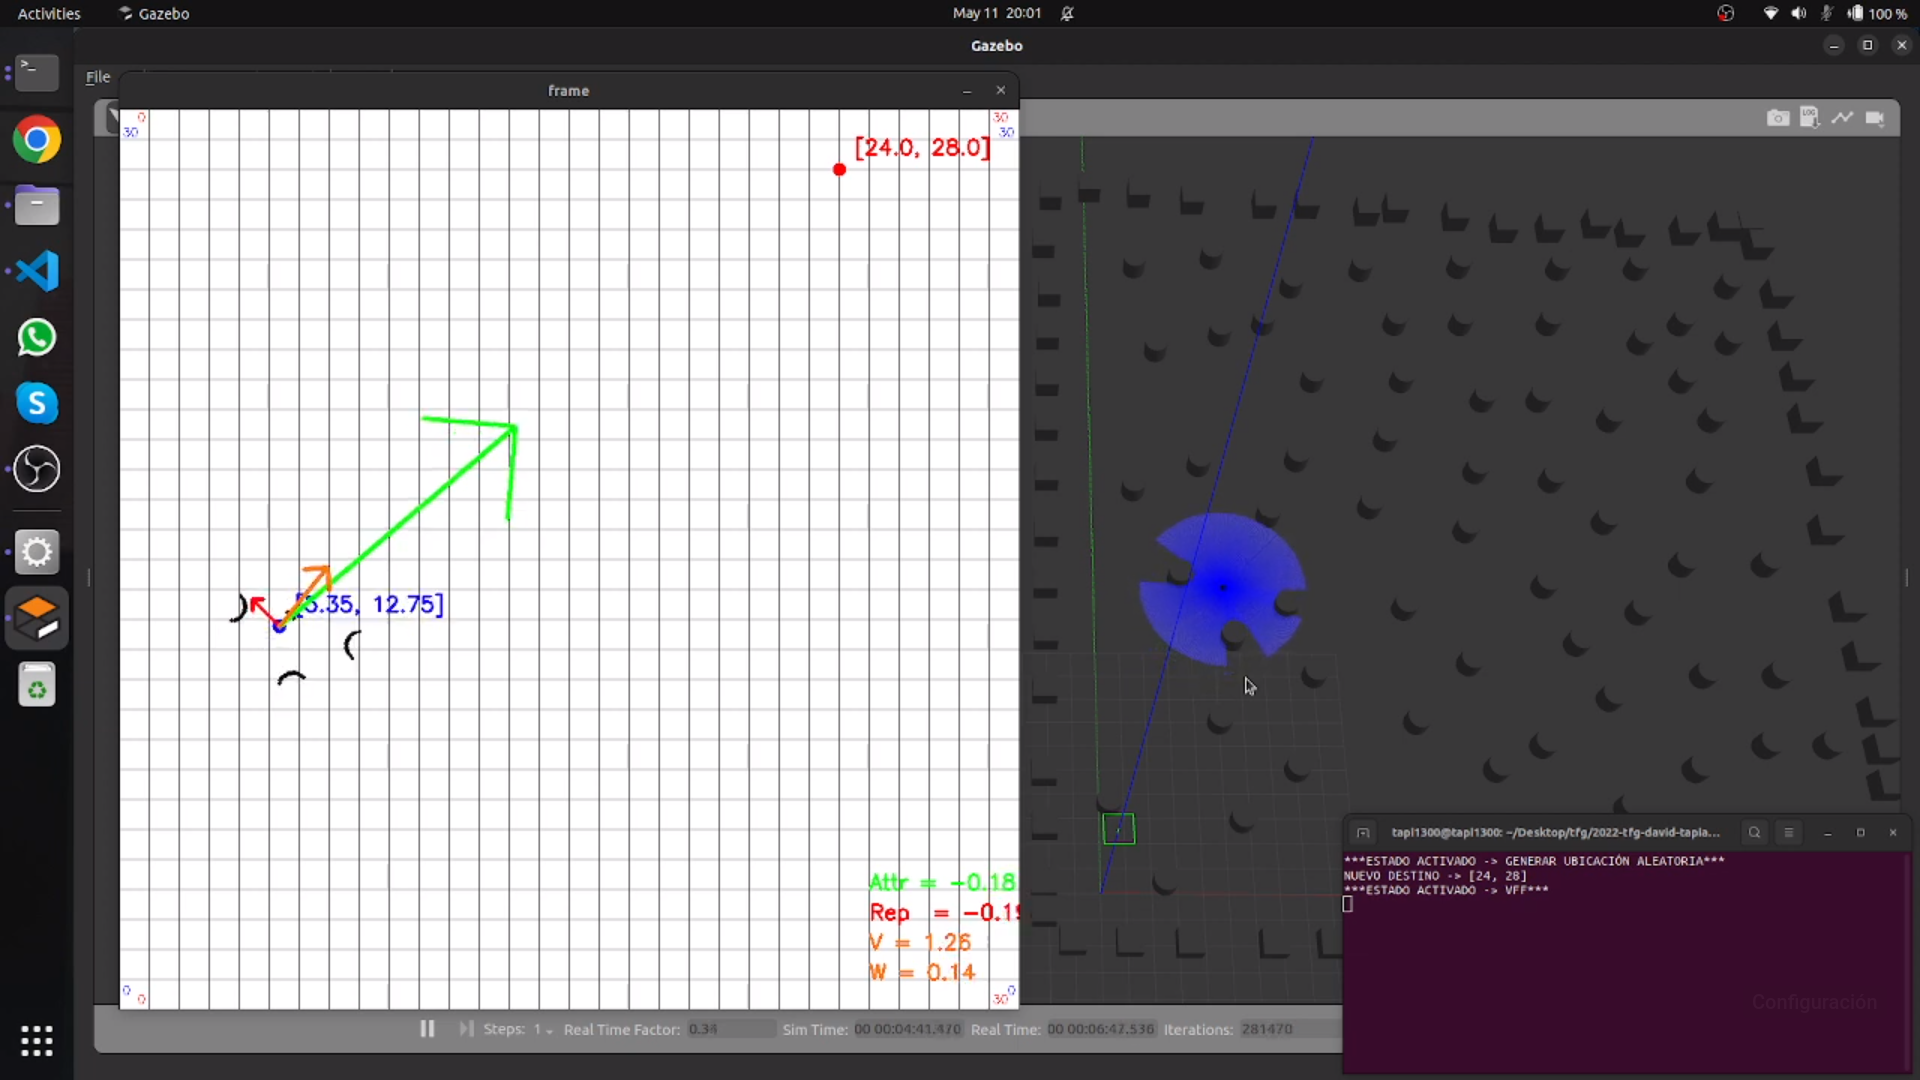
\includegraphics[width=7cm]{figs/c6/FSM_final1.png}
        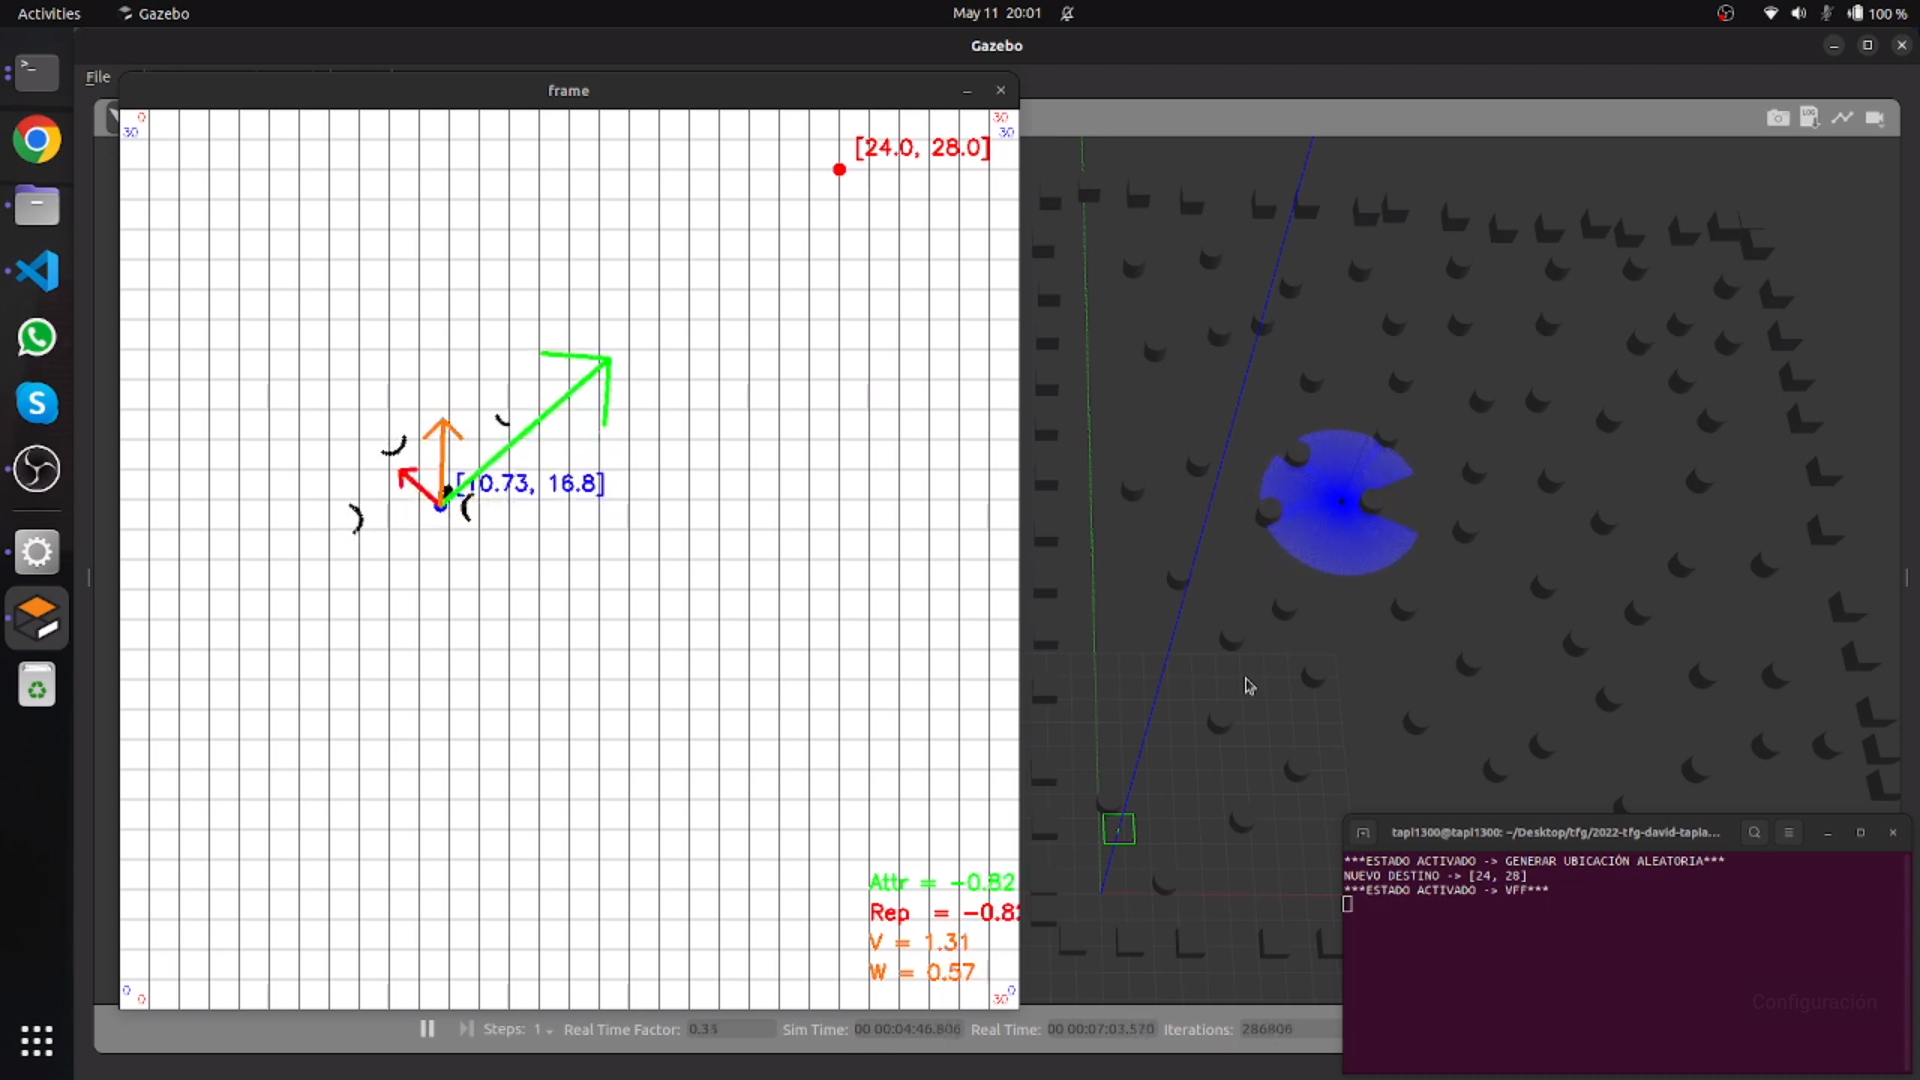
\includegraphics[width=7cm]{figs/c6/FSM_final2.png}
        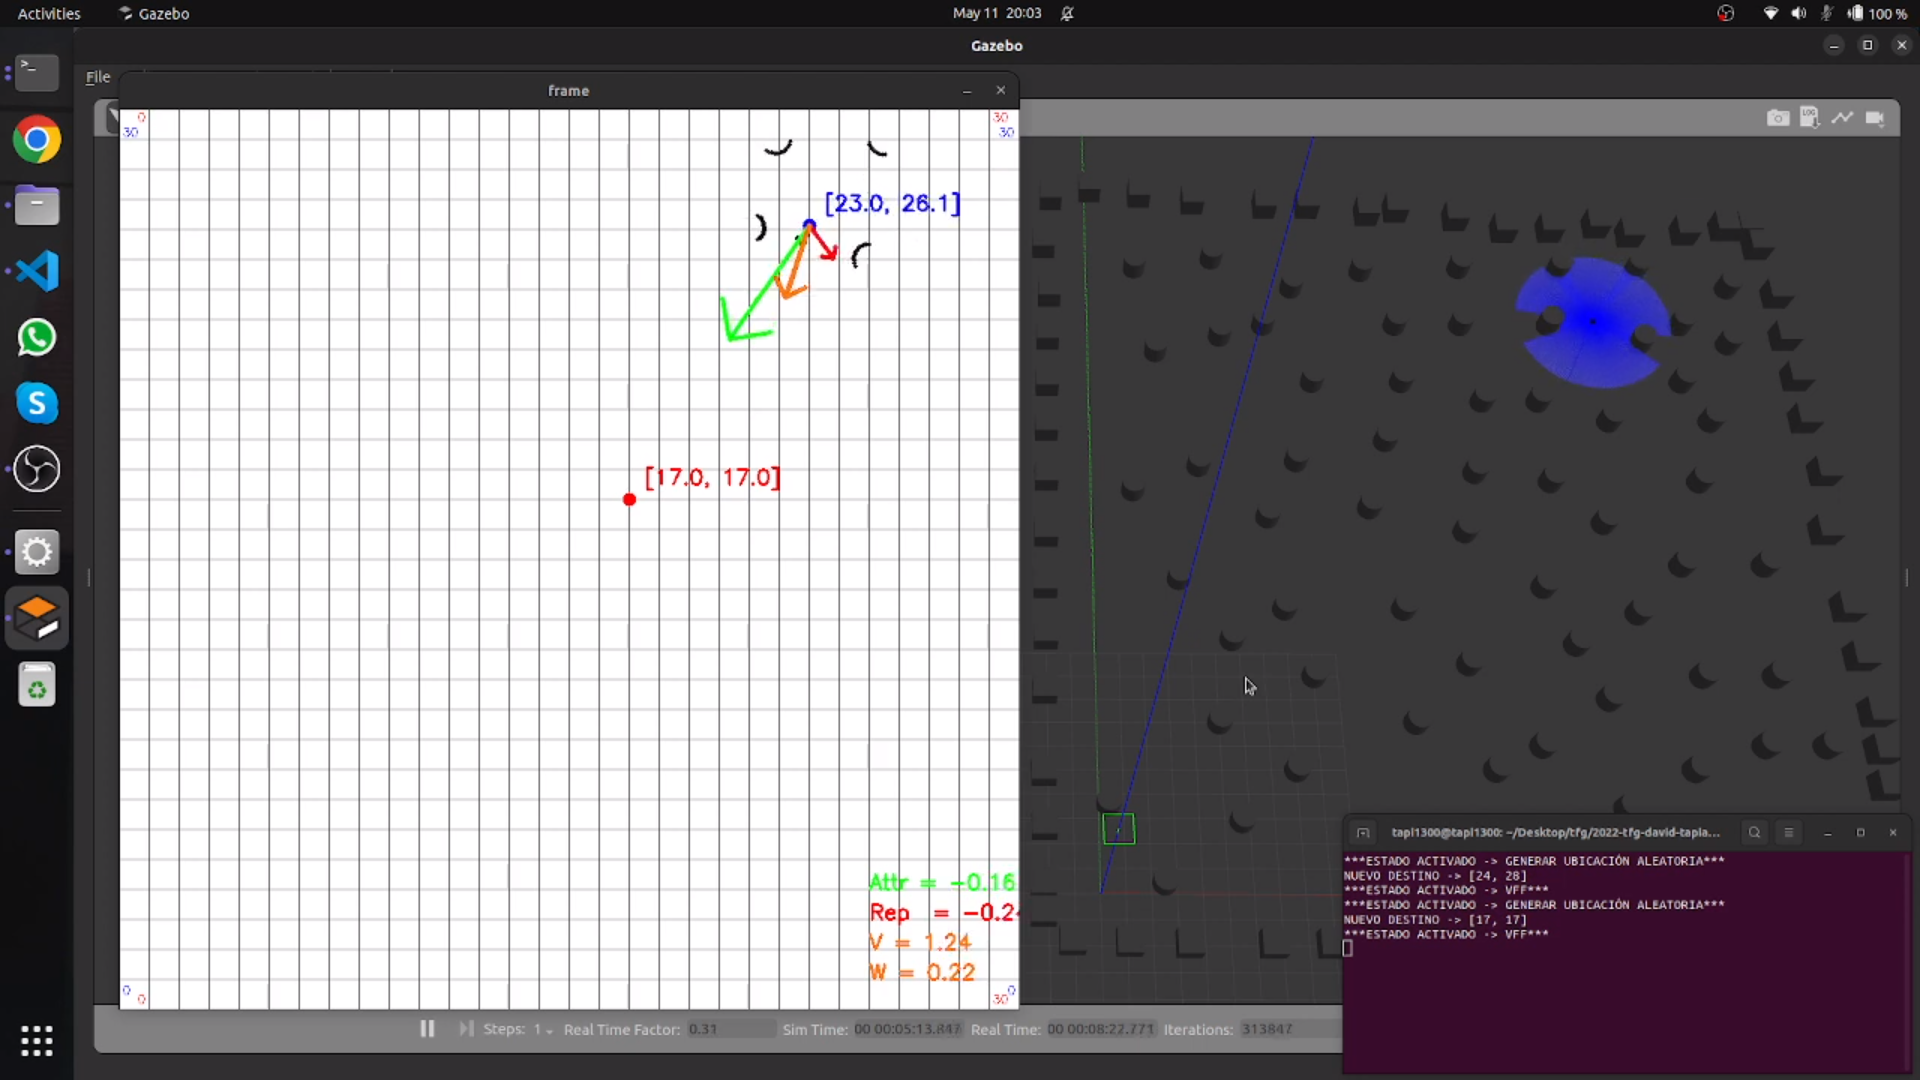
\includegraphics[width=7cm]{figs/c6/FSM_final3.png}
        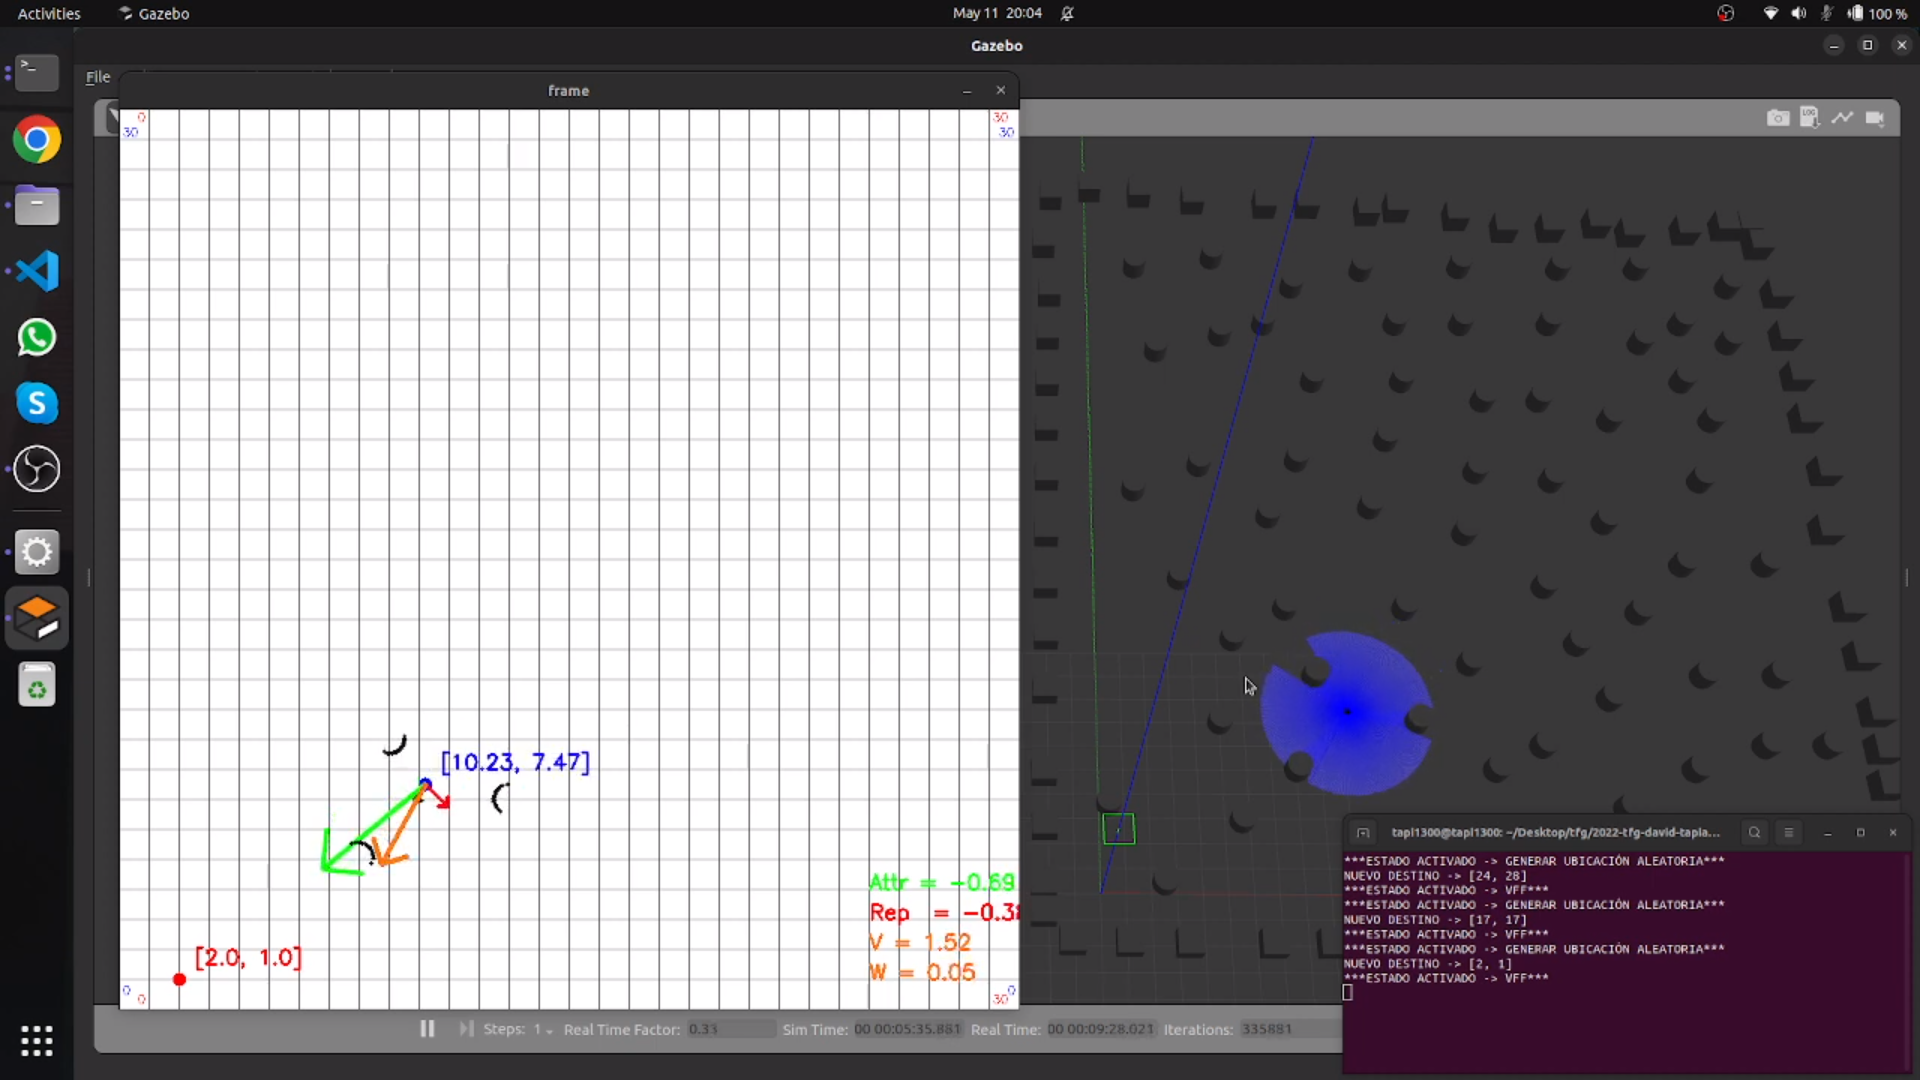
\includegraphics[width=7cm]{figs/c6/FSM_final4.png}
    \end{center}
    \caption[Secuencia VFF con FSM]{Secuencia de imágenes del algoritmo VFF usando FSM. Imagenes obtenidas de Youtube\footnotemark.}
    \label{fig:sec_FSM_final}
\end{figure}
\footnotetext{\textbf{Vídeo}: \url{https://www.youtube.com/watch?v=EiBT8yqX29Q&ab_channel=Tapii}}





